% !Mode:: "TeX:UTF-8"

\def\usewhat{pdflatex} % 定义编译方式 pdflatex, dvipdfmx, or xelatex

\def \xuewei{Bachelor} % 定义学位 Doctor, Master or Bachelor

\def\xueke{Engineering} % 定义学科 Engineering, Science, Management, Arts, Philosophy, Economics, Laws, Education, or History

\documentclass[cs4size,openany,twoside,UTF8]{ctexbook}

\input{setup/type.tex}    % 硕博类型
% !Mode:: "TeX:UTF-8" 

\usepackage{verbatim}
\usepackage{graphicx}
\usepackage[a4paper,text={150true mm,224true mm},top=35.5true mm,left=30true mm,head=5true mm,headsep=2.5true mm,foot=8.5true mm]{geometry}
\usepackage{titlesec}               % 控制标题的宏包
\usepackage{titletoc}                   % 控制目录的宏包
\usepackage{fancyhdr}                   % fancyhdr宏包 页眉和页脚的相关定义
\usepackage{color}          % 支持彩色
\usepackage{amsmath}        % AMSLaTeX宏包 用来排出更加漂亮的公式
\usepackage{amssymb}
%\usepackage[below]{placeins}%允许上一个section的浮动图形出现在下一个section的开始部分,还提供\FloatBarrier命令,使所有未处理的浮动图形立即被处理
%\usepackage{flafter}       % 使得所有浮动体不能被放置在其浮动环境之前,以免浮动体在引述它的文本之前出现.
\usepackage[export]{adjustbox}
\usepackage{multirow}       %使用Multirow宏包,使得表格可以合并多个row格
\usepackage{booktabs}       % 表格,横的粗线;\specialrule{1pt}{0pt}{0pt}
\usepackage{longtable}      %支持跨页的表格。
% \usepackage{tabularx}
\usepackage{makecell}
\usepackage[hang]{subfigure}%支持子图 %centerlast 设置最后一行是否居中
\usepackage[subfigure]{ccaption} %支持双语标题
\usepackage[sort&compress,numbers]{natbib}% 支持引用缩写的宏包
\usepackage{enumitem}       %使用enumitem宏包,改变列表项的格式
\usepackage{calc}           %长度可以用+ - * / 进行计算
\usepackage{txfonts}

\usepackage[hyphens]{url}

\usepackage{float}

\usepackage[amsmath,thmmarks,hyperref]{ntheorem}% 定理类环境宏包,其中 amsmath 选项用来兼容 AMS LaTeX 的宏包

% 生成有书签的pdf及其开关, 该宏包应放在所有宏包的最后, 宏包之间有冲突
\def\atemp{dvipdfmx}\ifx\atemp\usewhat
\usepackage[dvipdfmx,unicode,           %dvi-->pdf 生成书签
            bookmarksnumbered=true,
            bookmarksopen=true,
            colorlinks=false,
            pdfborder={0 0 1},
            citecolor=blue,
            linkcolor=red,
            anchorcolor=green,
            urlcolor=blue,
            breaklinks=true
            ]{hyperref}
\fi

\def\atemp{pdflatex}\ifx\atemp\usewhat
\usepackage{cmap}                       %pdflatex编译时,可以生成可复制、粘贴的中文PDF文档
\usepackage[pdftex,unicode,
            %CJKbookmarks=true,
            bookmarksnumbered=true,
            bookmarksopen=true,
            colorlinks=false,
            pdfborder={0 0 1},
            citecolor=blue,
            linkcolor=red,
            anchorcolor=green,
            urlcolor=blue,
            breaklinks=true
            ]{hyperref}
\fi

\def\atempxetex{xelatex}\ifx\atempxetex\usewhat %\def\atempxetex{xelatex} main.tex中已定义;
\usepackage[xetex,
            bookmarksnumbered=true,
            bookmarksopen=true,
            colorlinks=false,
            pdfborder={0 0 1},
            citecolor=blue,
            linkcolor=red,
            anchorcolor=green,
            urlcolor=blue,
            breaklinks=true,
            naturalnames  %与algorithm2e宏包协调
            ]{hyperref}
\fi

\usepackage[boxed,linesnumbered,algochapter]{algorithm2e}  % 算法的宏包,注意宏包兼容性,先后顺序为float、hyperref、algorithm(2e),否则无法生成算法列表
 % 引用的宏包

\graphicspath{{figures/}} %定义所有的eps文件在 figures 子目录下

%个人自定义的符号
\DeclareMathOperator{\similarity}{sim}

\begin{document}

% !Mode:: "TeX:UTF-8" 

\newcommand{\song}{\CJKfamily{song}}    % 宋体   (Windows自带simsun.ttf)
\newcommand{\fs}{\CJKfamily{fs}}        % 仿宋体 (Windows自带simfs.ttf)
\newcommand{\kai}{\CJKfamily{kai}}      % 楷体   (Windows自带simkai.ttf)
\newcommand{\hei}{\CJKfamily{hei}}      % 黑体   (Windows自带simhei.ttf)
\newcommand{\li}{\CJKfamily{li}}        % 隶书   (Windows自带simli.ttf)

%\ifxueweibachelor
%\setCJKfamilyfont{xwei}{STXinwei} 
%\newcommand{\xinwei}{\CJKfamily{xwei}} %华文新魏  系统不自带,本科封面蛋疼字体
%\fi

\newcommand{\chuhao}{\fontsize{42pt}{42pt}\selectfont}        % 初号, 单倍行距  本科蛋疼
\newcommand{\yihao}{\fontsize{26pt}{26pt}\selectfont}       % 一号, 1.倍行距
\newcommand{\xiaoyi}{\fontsize{24pt}{24pt}\selectfont}      % 小一, 1.倍行距
\newcommand{\erhao}{\fontsize{22pt}{1.25\baselineskip}\selectfont}       % 二号, 1.倍行距
\newcommand{\xiaoer}{\fontsize{18pt}{18pt}\selectfont}      % 小二, 单倍行距
\newcommand{\sanhao}{\fontsize{16pt}{16pt}\selectfont}      % 三号, 1.倍行距
\newcommand{\xiaosan}{\fontsize{15pt}{15pt}\selectfont}     % 小三, 1.倍行距
\newcommand{\sihao}{\fontsize{14pt}{14pt}\selectfont}       % 四号, 1.0倍行距
\newcommand{\xiaosi}{\fontsize{12pt}{12pt}\selectfont}      % 小四, 1.倍行距
\newcommand{\wuhao}{\fontsize{10.5pt}{10.5pt}\selectfont}   % 五号, 单倍行距
\newcommand{\xiaowu}{\fontsize{9pt}{9pt}\selectfont}        % 小五, 单倍行距


%避免宏包 hyperref 和 arydshln 不兼容带来的目录链接失效的问题。
\def\temp{\relax}
\let\temp\addcontentsline
\gdef\addcontentsline{\phantomsection\temp}

\makeatletter
\gdef\hitempty{}

%重新定义BiChapter命令,可实现标题手动换行,但不影响目录
\def\BiChapter{\relax\@ifnextchar [{\@BiChapter}{\@@BiChapter}}
\def\@BiChapter[#1]#2#3{\chapter[#1]{#2}
    \addcontentsline{toe}{chapter}{\bfseries \xiaosi Chapter \thechapter\hspace{0.5em} #3}}
\def\@@BiChapter#1#2{\chapter{#1}
    \addcontentsline{toe}{chapter}{\bfseries \xiaosi Chapter \thechapter\hspace{0.5em}{\boldmath #2}}}

\newcommand{\BiSection}[2]
{   \section{#1}
    \addcontentsline{toe}{section}{\protect\numberline{\csname thesection\endcsname}#2}
}

\newcommand{\BiSubsection}[2]
{    \subsection{#1}
    \addcontentsline{toe}{subsection}{\protect\numberline{\csname thesubsection\endcsname}#2}
}

\newcommand{\BiSubsubsection}[2]
{    \subsubsection{#1}
    \addcontentsline{toe}{subsubsection}{\protect\numberline{\csname thesubsubsection\endcsname}#2}
}

\newcommand{\BiAppendixChapter}[2] % 该附录命令适用于发表文章,简历等
{\phantomsection
\markboth{#1}{#1}
\addcontentsline{toc}{chapter}{\xiaosi #1}
\addcontentsline{toe}{chapter}{\bfseries \xiaosi #2}  \chapter*{#1}
}

\newcommand{\BiAuthorization}{
\phantomsection
\markboth{哈尔滨工业大学本科毕业设计(论文)原创性声明}{哈尔滨工业大学本科毕业设计(论文)原创性声明}
\addcontentsline{toc}{chapter}{\xiaosi 原创性声明}
\addcontentsline{toe}{chapter}{\bfseries \xiaosi Statement of copyright}  \chapter*{哈尔滨工业大学本科毕业设计(论文)原创性声明}	
}

\newcommand{\BiAppChapter}[2]    % 该附录命令适用于有章节的完整附录
{\phantomsection 
 \chapter{#1}
 \addcontentsline{toe}{chapter}{\bfseries \xiaosi Appendix \thechapter~~#2}
}

\renewcommand{\thefigure}{\arabic{chapter}-\arabic{figure}}%使图编号为 7-1 的格式 %\protect{~}
\renewcommand{\thesubfigure}{\alph{subfigure})}%使子图编号为 a)的格式
\renewcommand{\p@subfigure}{\thefigure~} %使子图引用为 7-1 a) 的格式,母图编号和子图编号之间用~加一个空格
\renewcommand{\thetable}{\arabic{chapter}-\arabic{table}}%使表编号为 7-1 的格式
\renewcommand{\theequation}{\arabic{chapter}-\arabic{equation}}%使公式编号为 7-1 的格式



\newcommand{\algoenname}{Algo.} %算法英文标题
\newfloatlist[chapter]{algoen}{aen}{\listalgoenname}{\algoenname}
\newfixedcaption{\algoencaption}{algoen}
\renewcommand{\thealgoen}{\thechapter-\arabic{algocf}}
\renewcommand{\@cftmakeaentitle}{\chapter*{\listalgoenname\@mkboth{\bfseries\listalgoenname}{\bfseries\listalgoenname}}}

\renewcommand{\algorithmcfname}{算法}
\setlength\AlCapSkip{1.2ex}
\SetAlgoSkip{1pt}
\renewcommand{\algocf@captiontext}[2]{\wuhao#1\algocf@typo ~ \AlCapFnt{}#2} % text of caption
\expandafter\ifx\csname algocf@within\endcsname\relax% if \algocf@within doesn't exist
\renewcommand\thealgocf{\@arabic\c@algocf} % and the way it is printed
\else%                                    else
\renewcommand\thealgocf{\csname the\algocf@within\endcsname-\@arabic\c@algocf}
\fi
\renewcommand{\algocf@makecaption}[2]{%中英文双标题一定多于一行,因此去掉单行时的判断,并将\parbox中标题设置为居中
  \addtolength{\hsize}{\algomargin}%
  \sbox\@tempboxa{\algocf@captiontext{#1}{#2}}%
    \hskip .5\algomargin%
    \parbox[t]{\hsize}{\centering\algocf@captiontext{#1}{#2}}% 
  \addtolength{\hsize}{-\algomargin}%
}
\newcommand{\AlgoBiCaption}[2]{%直接取出自定义的中英文标题条目加入到真正的\caption 中  
   \caption[#1]{\protect\setlength{\baselineskip}{1.5em}#1 \protect \\ Algo. \thealgocf~~ #2} % \algoencaption{#2}   
   \addcontentsline{aen}{algoen}{\protect\numberline{\thealgoen}{#2}}
   }

\makeatother

%定义 学科 学位
\def \xuekeEngineering {Engineering}
\def \xuekeScience {Science}
\def \xuekeManagement {Management}
\def \xuekeArts {Arts}
\def \xuekePhilosophy {Philosophy}
\def \xuekeEconomics {Economics}
\def \xuekeLaws {Laws}
\def \xuekeEducation {Education}
\def \xuekeHistory {History}


\ifx \xueke \xuekeEngineering
\newcommand{\cxueke}{工学}
\newcommand{\exueke}{Engineering}
\fi

\ifx \xueke \xuekeScience
\newcommand{\cxueke}{理学}
\newcommand{\exueke}{Science}
\fi

\ifx \xueke \xuekeManagement
\newcommand{\cxueke}{管理学}
\newcommand{\exueke}{Management}
\fi

\ifx \xueke \xuekeArts
\newcommand{\cxueke}{文学}
\newcommand{\exueke}{Arts}
\fi 

\ifx \xueke \xuekePhilosophy
\newcommand{\cxueke}{哲学}
\newcommand{\exueke}{Philosophy}
\fi 

\ifx \xueke \xuekeEconomics
\newcommand{\cxueke}{经济学}
\newcommand{\exueke}{Economics}
\fi 

\ifx \xueke \xuekeLaws
\newcommand{\cxueke}{法学}
\newcommand{\exueke}{Laws}
\fi 

\ifx \xueke \xuekeEducation
\newcommand{\cxueke}{教育学}
\newcommand{\exueke}{Education}
\fi 

\ifx \xueke \xuekeHistory
\newcommand{\cxueke}{历史学}
\newcommand{\exueke}{History}
\fi 
 % 文本格式定义

\frontmatter
\ifxueweibachelor
  % !Mode:: "TeX:UTF-8" 

\theoremstyle{plain}
\theorembodyfont{\song\rmfamily}
\theoremheaderfont{\hei\rmfamily}
\newtheorem{definition}{\hei 定义}[chapter]
\newtheorem{example}{\hei 例}[chapter]
\newtheorem{algo}{\hei 算法}[chapter]
\newtheorem{theorem}{\hei 定理}[chapter]
\newtheorem{axiom}{\hei 公理}[chapter]
\newtheorem{proposition}{\hei 命题}[chapter]
\newtheorem{lemma}{\hei 引理}[chapter]
\newtheorem{corollary}{\hei 推论}[chapter]
\newtheorem{remark}{\hei 注解}[chapter]
\newenvironment{proof}{\noindent{\hei 证明:}}{\hfill $ \square $ \vskip 4mm}
\theoremsymbol{$\square$}
\setlength{\theorempreskipamount}{0pt}
\setlength{\theorempostskipamount}{-2pt}

\allowdisplaybreaks[4]

\CJKcaption{gb_452} 
\CJKtilde
\setlength{\parindent}{2em}

\arraycolsep=1.6pt

\renewcommand\contentsname{\hei 目~~~~录}

\renewcommand\chaptername{\CJKprechaptername~\thechapter~\CJKchaptername}

\setcounter{secnumdepth}{4} \setcounter{tocdepth}{2}


\titleformat{\chapter}{\center\xiaoer\hei}{\chaptertitlename}{0.5em}{}
\titlespacing{\chapter}{0pt}{-5.5mm}{8mm}
\titleformat{\section}{\xiaosan\hei}{\thesection}{0.5em}{}
\titlespacing{\section}{0pt}{4.5mm}{4.5mm}
\titleformat{\subsection}{\sihao\hei}{\thesubsection}{0.5em}{}
\titlespacing{\subsection}{0pt}{4mm}{4mm}
\titleformat{\subsubsection}{\xiaosi\hei}{\thesubsubsection}{0.5em}{}
\titlespacing{\subsubsection}{0pt}{0pt}{0pt}

\titlecontents{chapter}[3.8em]{\hspace{-3.8em}\hei}{\CJKprechaptername~\thecontentslabel~\CJKchaptername~~}{}{\titlerule*[4pt]{.}\contentspage}
\dottedcontents{section}[32pt]{}{21pt}{0.3pc}
\dottedcontents{subsection}[53pt]{}{30pt}{0.3pc}


% 按工大标准, 缩小目录中各级标题之间的缩进,使它们相隔一个字符距离,也就是12pt
\makeatletter
\renewcommand*\l@chapter{\@dottedtocline{0}{0em}{5em}}%控制英文目录: 细点\@dottedtocline  粗点\@dottedtoclinebold
\renewcommand*\l@section{\@dottedtocline{1}{1em}{1.8em}}
\renewcommand*\l@subsection{\@dottedtocline{2}{2em}{2.5em}}


% 定义页眉和页脚
\newcommand{\makeheadrule}{
\rule[7pt]{\textwidth}{0.75pt} \\[-23pt]
\rule{\textwidth}{2.25pt}}
\renewcommand{\headrule}{
    {\if@fancyplain\let\headrulewidth\plainheadrulewidth\fi
     \makeheadrule}}
\pagestyle{fancyplain}

%去掉章节标题中的数字
%%不要注销这一行,否则页眉会变成:“第1章1  绪论”样式
\renewcommand{\chaptermark}[1]{\markboth{\chaptertitlename~\ #1}{}}
\fancyhf{}

%在book文件类别下,\leftmark自动存录各章之章名,\rightmark记录节标题
%% 页眉字号 工大要求 小五
%根据单双面打印设置不同的页眉;

\ifxueweidoctor
  \fancyhead[CO]{\song \xiaowu\leftmark}
  \fancyhead[CE]{\song \xiaowu 哈尔滨工业大学\cxueke\cxuewei 学位论文 }%
  \fancyfoot[C,C]{\xiaowu -~\thepage~-}
\else
  \ifxueweimaster
    \fancyhead[CO]{\song \xiaowu 哈尔滨工业大学\cxueke\cxuewei 学位论文}
    \fancyhead[CE]{\song \xiaowu 哈尔滨工业大学\cxueke\cxuewei 学位论文}%
    \fancyfoot[C,C]{\xiaowu -~\thepage~-}
  \else
    \fancyhead[CO]{\song \xiaowu 哈尔滨工业大学本科毕业设计(论文)}
    \fancyhead[CE]{\song \xiaowu 哈尔滨工业大学本科毕业设计(论文)}%
    \fancyfoot[C,C]{\xiaowu -~\thepage~-}
  \fi
\fi

\renewcommand\frontmatter{\cleardoublepage
  \@mainmatterfalse
  \pagenumbering{Roman}}

% 调整罗列环境的布局
\setitemize{leftmargin=0em,itemsep=0em,partopsep=0em,parsep=0em,topsep=0em,itemindent=3em}
\setenumerate{leftmargin=0em,itemsep=0em,partopsep=0em,parsep=0em,topsep=0em,itemindent=3.5em}

\newcommand{\citeup}[1]{\textsuperscript{\cite{#1}}}

% 定制浮动图形和表格标题样式
\captionnamefont{\wuhao}
\captiontitlefont{\wuhao}
\captiondelim{~~}
%\captionstyle{\hang}
\hangcaption
\renewcommand{\subcapsize}{\wuhao}
\setlength{\abovecaptionskip}{0pt}
\setlength{\belowcaptionskip}{0pt}

% 自定义项目列表标签及格式 \begin{publist} 列表项 \end{publist}
\newcounter{pubctr} %自定义新计数器
\newenvironment{publist}{%%%%%定义新环境
\begin{list}{[\arabic{pubctr}]} %%标签格式
    {
     \usecounter{pubctr}
     \setlength{\leftmargin}{1.7em}     % 左边界 \leftmargin =\itemindent + \labelwidth + \labelsep
     \setlength{\itemindent}{0em}     % 标号缩进量
     \setlength{\labelsep}{0.5em}       % 标号和列表项之间的距离,默认0.5em
     \setlength{\rightmargin}{0em}    % 右边界
     \setlength{\topsep}{0ex}         % 列表到上下文的垂直距离
     \setlength{\parsep}{0ex}         % 段落间距
     \setlength{\itemsep}{0ex}        % 标签间距
     \setlength{\listparindent}{0pt} % 段落缩进量
    }}
{\end{list}}%%%%%

% 默认字体
\renewcommand\normalsize{
  \@setfontsize\normalsize{12pt}{12pt}
  \setlength\abovedisplayskip{4pt}
  \setlength\abovedisplayshortskip{4pt}
  \setlength\belowdisplayskip{\abovedisplayskip}
  \setlength\belowdisplayshortskip{\abovedisplayshortskip}
  \let\@listi\@listI}
  
% 设置行距和段落间垂直距离
\def\defaultfont{\renewcommand{\baselinestretch}{1.62}\normalsize\selectfont}
\renewcommand{\CJKglue}{\hskip 0.56pt plus 0.08\baselineskip} 
%加大字间距,使每行34个字,若要使得每行33个字,则将0.56pt替换为0.96pt。
\predisplaypenalty=0  %公式之前可以换页,公式出现在页面顶部

% 封面、摘要、版权、致谢格式定义
\def\ctitle#1{\def\@ctitle{#1}}\def\@ctitle{}
\def\ctitleone#1{\def\@ctitleone{#1}}\def\@ctitleone{}
\def\ctitletwo#1{\def\@ctitletwo{#1}}\def\@ctitletwo{}
\def\cdegree#1{\def\@cdegree{#1}}\def\@cdegree{}
\def\caffil#1{\def\@caffil{#1}}\def\@caffil{}
\def\csubject#1{\def\@csubject{#1}}\def\@csubject{}
\def\cauthor#1{\def\@cauthor{#1}}\def\@cauthor{}
\def\cstuid#1{\def\@cstuid{#1}}\def\@cstuid{} % 本科蛋疼学号
\def\csupervisor#1{\def\@csupervisor{#1}}\def\@csupervisor{}
\def\cassosupervisor#1{\def\@cassosupervisor{{\hei 副 \hfill 导 \hfill 师} & #1\\}}\def\@cassosupervisor{}
\def\ccosupervisor#1{\def\@ccosupervisor{{\hei 联 \hfill 合\hfill 导 \hfill 师} & #1\\}}\def\@ccosupervisor{}
\def\cdate#1{\def\@cdate{#1}}\def\@cdate{}
\def\cmonth#1{\def\@cmonth{#1}}\def\@cmonth{}
\long\def\cabstract#1{\long\def\@cabstract{#1}}\long\def\@cabstract{}
\def\ckeywords#1{\def\@ckeywords{#1}}\def\@ckeywords{}

\def\etitle#1{\def\@etitle{#1}}\def\@etitle{}
\def\edegree#1{\def\@edegree{#1}}\def\@edegree{}
\def\eaffil#1{\def\@eaffil{#1}}\def\@eaffil{}
\def\esubject#1{\def\@esubject{#1}}\def\@esubject{}
\def\eauthor#1{\def\@eauthor{#1}}\def\@eauthor{}
\def\esupervisor#1{\def\@esupervisor{#1}}\def\@esupervisor{}
\def\eassosupervisor#1{\def\@eassosupervisor{\textbf{Associate Supervisor:} & #1\\}}\def\@eassosupervisor{}
\def\ecosupervisor#1{\def\@ecosupervisor{\textbf{Co Supervisor:} & #1\\}}\def\@ecosupervisor{}
\def\edate#1{\def\@edate{#1}}\def\@edate{}
\long\def\eabstract#1{\long\def\@eabstract{#1}}\long\def\@eabstract{}
\long\def\NotationList#1{\long\def\@NotationList{#1}}\long\def\@NotationList{}
\def\ekeywords#1{\def\@ekeywords{#1}}\def\@ekeywords{}
\def\natclassifiedindex#1{\def\@natclassifiedindex{#1}}\def\@natclassifiedindex{}
\def\internatclassifiedindex#1{\def\@internatclassifiedindex{#1}}\def\@internatclassifiedindex{}
\def\statesecrets#1{\def\@statesecrets{#1}}\def\@statesecrets{}

% 定义封面
\def\makecover{
    \begin{titlepage}
    % 封面一
   \vspace*{0.8cm}
   \begin{center}
   
    \parbox[t][3.4cm][t]{\textwidth}{
    \begin{center}\erhao\hei\@ctitle\end{center} }
    
    \parbox[t][9.4cm][t]{\textwidth}{
        \begin{center}\xiaoer\song\textbf{\@cauthor}\end{center}}
  
      
            {\hei \xiaosi
 			\begin{tabular*}{6.768cm}{@{}r@{:}c@{}}
 			院\hfill(系) & \@caffil\\[14pt]
  			学\quad \quad 号 & \@cstuid
 			\end{tabular*}}
 			{\hei \xiaosi
 			\begin{tabular*}{6.768cm}{@{}r@{:}c@{}}
 			专\hfill业 & \@csubject\\[14pt]
  			指导教师 &  \@csupervisor
 			\end{tabular*}}

    \vspace*{3.0cm}
    
    {\song\xiaosi\textbf{\@cmonth}}

    \end{center}

    %内封
    \newpage
    \thispagestyle{empty}

\begin{center}

	\vspace*{0.6cm}
	
   % \parbox[t][3.2cm][t]{\textwidth}{\begin{center} \end{center} }
    
    \begin{figure}[htbp]
   	\centering
   	\includegraphics[scale=0.38]{logo.jpg}
   	\end{figure}
   	
   	\vspace*{0.75cm}
   	
   	%{\kai\chuhao\textbf{毕业设计(论文)}} % 字体等待替换中
   	
   	 %教务处去死吧,不知道华文新魏是付费的吗你妹,呵呵!先上图!
   	\begin{figure}[htbp]
	\centering
	\includegraphics[scale=0.25]{hehejwc.png}
	\end{figure}
	
    \vspace*{1.7cm}
    
	\parbox[t][14.2cm][b]{\textwidth}
     {\xiaosan
    \begin{center} \renewcommand{\arraystretch}{2.5} \hei
    \begin{tabular}{l@{\ \  }c}
    {\hei\xiaoer  题\hfill 目}                  & \underline{\makebox[6.1cm]{\xiaoer \@ctitleone}}\\
    &  \underline{\makebox[6.1cm]{\xiaoer \@ctitletwo}}\\
	& \\
    {\hei 专\hfill 业}                  & \underline{\makebox[6.1cm]{\@csubject}}\\
    {\hei 学\hfill 号}                  & \underline{\makebox[6.1cm]{\@cstuid}}\\
    {\hei 学\hfill 生}                  & \underline{\makebox[6.1cm]{\@cauthor}}\\
    {\hei 指\hfill 导\hfill 教\hfill 师} & \underline{\makebox[6.1cm]{\@csupervisor}}\\
    {\hei 答\ \  \hfill 辩\ \  \hfill 日\ \  \hfill 期} & \underline{\makebox[6.1cm]{\@cdate}}
    \end{tabular} \renewcommand{\arraystretch}{1}
    \end{center} }
\end{center}

    \end{titlepage}

%%%%%%%%%%%%%%%%%%%   Abstract and keywords  %%%%%%%%%%%%%%%%%%%%%%%
\clearpage

\BiAppendixChapter{摘\quad 要}{Abstract (In Chinese)}

\setcounter{page}{1}
\song\defaultfont
\@cabstract
\vspace{\baselineskip}

\hangafter=1\hangindent=51pt\noindent
{\hei 关键词}:\@ckeywords

%%%%%%%%%%%%%%%%%%%   English Abstract  %%%%%%%%%%%%%%%%%%%%%%%%%%%%%%
\clearpage

\phantomsection
\markboth{Abstract}{Abstract}
\addcontentsline{toc}{chapter}{\xiaosi ABSTRACT}
\addcontentsline{toe}{chapter}{\bfseries \xiaosi Abstract (In English)}  \chapter*{Abstract}
\@eabstract
\vspace{\baselineskip}

\hangafter=1\hangindent=60pt\noindent
{\textbf{Keywords:}}  \@ekeywords
}

%%%%%%%%%%%%%%%%%%%%%%%%%%%%%%%%%%%%%%%%%%%%%%%%%%%%%%%%%%%%%%%
% 英文目录格式
\def\@dotsep{0.75}           % 定义英文目录的点间距
\setlength\leftmargini {0pt}
\setlength\leftmarginii {0pt}
\setlength\leftmarginiii {0pt}
\setlength\leftmarginiv {0pt}
\setlength\leftmarginv {0pt}
\setlength\leftmarginvi {0pt}

\def\engcontentsname{\bfseries Contents}
\newcommand\tableofengcontents{
   \pdfbookmark[0]{Contents}{econtent}
     \@restonecolfalse
   \chapter*{\engcontentsname  %chapter*上移一行,避免在toc中出现。
       \@mkboth{%
          \engcontentsname}{\engcontentsname}}
   \@starttoc{toe}%
   \if@restonecol\twocolumn\fi
   }

\urlstyle{same}  %论文中引用的网址的字体默认与正文中字体不一致,这里修正为一致的。

\renewcommand\endtable{\vspace{-4mm}\end@float}

\makeatother

% magic282 added some cmds here
\renewcommand{\subcapsize}{\centering\song\wuhao} % 为了使子图的长标题居中
 % 本科蛋疼格式
\else
  \input{setup/format} % 硕博格式
\fi

\frontmatter
\ifxueweibachelor
  % !Mode:: "TeX:UTF-8" 

\newcommand{\chinesethesistitle}{中文词语相似度计算} %授权书用,无需断行
%\newcommand{\englishthesistitle}{\uppercase{english title is undetermmined!}} %\uppercase作用:将英文标题字母全部大写;
\newcommand{\chinesethesistime}{2017 年 6 月 23 日}  %封面底部的日期中文形式


\ctitle{中文词语相似度计算}  %封面用论文标题,自己可手动断行
\ctitleone{中文词语} %用于内封上的两行标题,请手动根据标题内容酌情断行
\ctitletwo{相似度计算} %用于内封上的两行标题,请手动根据标题内容酌情断行
\cdegree{\cxueke\cxuewei}
\csubject{计算机科学与技术}                 %(~按二级学科填写~)
\caffil{计算机科学与技术学院} %(在校生填所在系名称,同等学力人员填工作单位)
\cauthor{周奇安}
\csupervisor{孙大烈} %导师名字
\cstuid{1130310402} %本科蛋疼学号


\cdate{\chinesethesistime}
\cmonth{2017 年 6 月}


\iffalse
\BiAppendixChapter{摘~~~~要}{}  %使用winedt编辑时文档结构图(toc)中为了显示摘要,故增加此句;
\fi
\cabstract{
中文词语相似度计算的目的是使用自动化的方法给出一个量化的指标,来衡量一对中文词语之间的相似程度。本课题取自 NLPCC-ICCPOL 2016 会议中一个开放任务。本文使用了深度学习的二分类方法、深度学习辅助词嵌入方法与基于词典或知识库的方法计算词语相似度,并使用集成学习方法结合其他方法的结果。

深度学习的二分类方法使用了生成替换句的手段,将无监督回归问题转化为有监督分类问题,并且使用深层 LSTM 的技术解决了分类问题。深度学习辅助词嵌入方法利用词嵌入计算词语相似度,并改进了现有的 ivLBL 方法,利用双向 LSTM 计算上下文向量。基于词典或知识库的方法从同义词词林扩展版中提取有用的特征用于计算。集成学习方法使用了 stacking 方法,并尝试了线性回归、岭回归与 LASSO 三种回归模型。

词语相似度计算方法的性能使用系统输出与人工标注间的 Spearman 等级相关系数来衡量。本文所介绍的方法可以得到 0.4855 的成绩。在不依赖 PKU-500 数据集的情况下,成绩也可以达到 0.3667。
}

\ckeywords{词语相似度;深度学习;LSTM;词嵌入;同义词词林;集成学习}

\eabstract{
Chinese word similarity measurement is a task aiming to provide a quantized measurement of the similarity of a pair of Chinese words. This project came from a shared task from the conference NLPCC-ICCPOL 2016. This thesis utilized deep learning classification method, deep learning aided word embedding method and dictionary / knowledge base based method to calculate word similarity. Then, ensemble learning method is used to combine results generated from other methods.

Deep learning classification method uses a means of generating word-replaced sentences to transform the unsupervised regression problem into a supervised classification problem. After that, deep LSTMs are used to solve the classification problem. Deep learning aided word embedding method makes use of word embedding to calculate word similarity. It improves the existing ivLBL method, calculating context vectors with bidirectional LSTMs. Dictionary / knowledge base based method extracts useful features from Tongyici Cilin (Extended). Ensemble learning uses stacking method, makes attempts with linear regression, ridge regression and LASSO.

The performance of word similarity measurement methods is measured by the Spearman's rank correlation coefficient between the system outputs and human annotations. The method introduced by this thesis achieved a performance of 0.4855. Even if not to depend on the PKU-500 dataset, the performance can reach 0.3667.
}

\ekeywords{word similarity, deep learning, LSTM, word embedding, Tongyici Cilin, ensemble learning}

\makecover
\clearpage  % 本科蛋疼封面
\else
  \input{cover} % 硕博封面
\fi

% 中英目录
\defaultfont
\clearpage{\pagestyle{empty}\cleardoublepage}
\pdfbookmark[0]{目~~~~录}{mulu}
\tableofcontents    % 中文目录
\clearpage{\pagestyle{empty}\cleardoublepage}

\ifxueweidoctor
\tableofengcontents % 英文目录
\clearpage{\pagestyle{empty}\cleardoublepage}     % 清除目录后面空页的页眉和页脚
\fi





\mainmatter\defaultfont\sloppy\raggedbottom

% !Mode:: "TeX:UTF-8"

\BiChapter{深度学习的二分类方法}{}
\label{c:classifer}
中文词语相似度计算本身是一个无监督的回归问题,这增加了解决问题的难度。如果能够将无监督学习转化为有监督学习,并且将回归问题转化为分类问题,就可以利用大量已知的模型,问题解决的难度也将会大大降低。

本章将介绍一种方法,这种方法利用词语在句子中的可替换性计算词语相似度。如果一个“通顺”的句子中的一个词语被替换之后,形成的句子仍然较为“通顺”,则本方法认为原词语和替换的词语较为接近;否则,认为两词语差距较大。本方法从未经处理的生语料库中抽取句子生成数据,并训练一个辅助的二分类器以判定句子的“通顺”与否。二分类器使用深度学习模型构建,以提高模型对整个句子的理解能力。

\BiSection{原理介绍}{}
\label{s:classifer pricinple}
为了更清晰的介绍深度学习的二分类方法,本文将先给出一些形式化的定义。

在深度学习的二分类方法中使用的语料库 $\mathcal{C}$ 是一个句子的多重集合,其中每一个句子是一个词语的序列,即:
\begin{equation}
\mathcal{C} \subset \mathcal{V}^+
\label{e:corpus}
\end{equation}
其中 $\mathcal{V}$ 是所有词语的集合。

替换函数 $f_\text{r}$ 可以将一个句子 $s \in \mathcal{C}$ 中的某个词语 $s_i$ 替换为一个不同的词语 $v \ne s_i$,即:
\begin{equation}
f_\text{r}(s, i, v) = (s_1, \dots, s_{i - 1}, v, s_{i + 1}, \dots, s_{|s|})
\end{equation}
对语料库中的句子应用替换函数 $f_\text{r}$ 得到的句子称为替换句:
\begin{equation}
\mathcal{C}_\text{r} = \bigl\{f_\text{r}(s, i, v) \bigm| s \in \mathcal{C}, v \in \mathcal{V}\bigr\}
\end{equation}
一般来说,$\mathcal{C}_\text{r} \cap \mathcal{C} \approx \emptyset$。本课题希望得到一个二分类器 $M_\mathcal{C}$,满足:
\begin{equation}
M_\mathcal{C}(s) = 
\begin{cases}
1 & s \in \mathcal{C}, \\
0 & s \in \mathcal{C}_\text{r}
\end{cases}
\end{equation}
使得 $M$ 可以区分原句与替换句。

利用这样的二分类器,我们就可以定义词语对 $(v_\text{a}, v_\text{b})$ 的相似度:
\begin{equation}
\similarity(w_\text{a}, w_\text{b}) = E\Bigl(M_\mathcal{C}\bigl(f_\text{r}(s, i, v_\text{b})\bigr) \Bigm| s \in \mathcal{C}, s_i = v_\text{a}\Bigr)
\label{e:avg}
\end{equation}
其中 $E$ 为数学期望。其中的思想是,利用包含词语 $v_\text{a}$ 的句子以 $v_\text{b}$ 替换得到的替换句测试二分类器 $M_\mathcal{C}$,若二分类器容易将这样的替换句误判为原句,则说明词语对 $(v_\text{a}, v_\text{b})$ 相似。为了提高准确性,应同时考虑从 $v_\text{a}$ 到 $v_\text{b}$ 和从 $v_\text{b}$ 到 $v_\text{a}$ 的替换。

\BiSubsection{训练数据生成}{}
为了训练二分类器 $M_\mathcal{C}$,我们需要一些带有标注的句子 $(x, y) \in \mathcal{V}^+ \times \{0, 1\}$ 作为训练数据。其中:
\begin{equation}
	y = 
	\begin{cases}
		1 & x \in \mathcal{C}, \\
		0 & x \in \mathcal{C}_\text{r}
	\end{cases}
\end{equation}
原句的生成是非常容易的,只需将 $M_\mathcal{C}$ 中全部的句子标注为 $1$ 即可。而替换句的生成需要一些额外的步骤。

利用随机采样的方法,我们可以生成一些采样句。采样句定义如下:
\begin{equation}
\mathcal{C}_\text{s} = \Bigl\{f_\text{r}(s, i, v) \Bigm| s \in \mathcal{C}, i \sim \mathcal{U}\bigl\{1, |s|\bigr\}, v \sim \mathcal{D}_\mathcal{V}\Bigr\}
\end{equation}
其中 $\mathcal{U}$ 为均匀分布,$\mathcal{D}_\mathcal{V}$ 为词语在自然语言中出现的概率分布。也就是说,采样句中的被替换词语位置 $i$ 是随机选择的,而替换词语 $v$ 亦是从词语分布中采样得到的。

显然,$\mathcal{C}_\text{s} \subset \mathcal{C}_\text{r}$,而随机采样对于计算机来说是轻而易举的任务。这样,我们就可以通过生成采样句的方式获得用于训练的替换句。

\BiSubsection{循环神经网络}{}
\label{s:classifer rnn}
上文提到,本课题需要训练一个二分类器 $M_\mathcal{C}$ 用于区分原句和替换句。二分类器的输入是一个句子 $x \in \mathcal{V}^+$,而输出为 $y' = M_\mathcal{C}(x) \in \{0, 1\}$。

循环神经网络(RNN)是一种具有循环连接的神经网络。这类神经网络可以用于进行时间序列的处理,因此常用于自然语言处理领域。

由于各类神经网络均以向量作为输入,因此需要将句子中的词语转化为向量,也就是词嵌入。词嵌入的形式非常简单,设有词嵌入矩阵 $E^{|\mathcal{V}| \times n_{\text{embed}}}$,则词嵌入的结果为:
\begin{equation}
e_i = E_{x_i}
\end{equation}
其中 $n_{\text{embed}}$ 是词嵌入维数。由于目前缺少成熟的预训练的中文词嵌入,所以本课题将词嵌入矩阵 $E$ 作为可训练参数,与网络参数同时接受优化算法的优化。

循环神经网络的结构如图 \ref{f:rnn} 所示。其中,$e_i$ 如上文所述,作为循环神经网络的输入,而 $h_i$ 是循环神经网络的输出。

\begin{figure}[h]
	\centering
	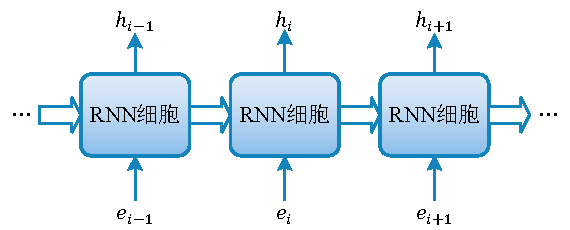
\includegraphics{RNN}
	\caption{RNN 结构}
	\label{f:rnn}
	\vspace{-1em}
\end{figure}

RNN 细胞可以看作是一个带有可训练参数的函数,每个 RNN 细胞的可训练参数共享。相邻的 RNN 细胞之间会传递一些信息,信息的内容取决于 RNN 细胞的种类。

\BiSubsection{LSTM}{}
\label{s:classifer lstm}
现代的循环神经网络具有多种变种,其中非常著名的一种即是 \cite{Hochreiter1997} 中提出的 LSTM (Long short-term memory)。其经过了 \cite{Gers2000} 改进,形成了现在常见的 LSTM 形式。本课题中即采用上述 LSTM 模型构建二分类器。

LSTM 与其它 RNN 的不同之处在于其独特的细胞结构,如图 \ref{f:lstm} 所示。LSTM 的最大特点是其优秀的“记忆能力”,即能处理时间序列中间隔很长的事件。这得益于 LSTM 中加入的遗忘门、输入门和输出门的设计。

\begin{figure}[h]
	\centering
	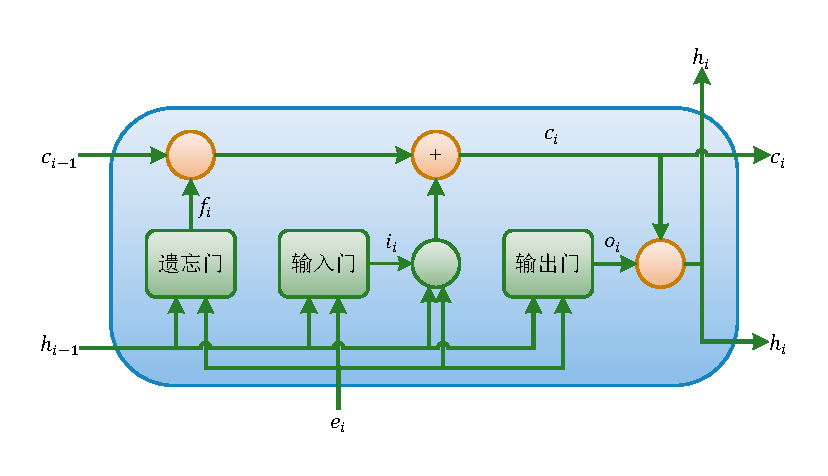
\includegraphics{LSTM}
	\caption{LSTM 细胞结构}
	\label{f:lstm}
	\vspace{-1em}
\end{figure}

图 \ref{f:lstm} 中的 $c_i$ 是 LSTM 细胞间的隐藏状态,$f_i$ 为遗忘门,$i_i$ 为输入门,$o_i$ 为输出门。公式 (\ref{e:lstm begin}) -- (\ref{e:lstm end}) 给出了一个 LSTM 细胞的完整定义,其中 $W$、$U$、$b$ 都是可训练参数,而 $\sigma$ 是 sigmoid 函数,$\circ$ 是逐项乘积。

\begin{align}
f_i &= \sigma(W_\text{f} e_i + U_\text{f} h_{i - 1} + b_\text{f}) \label{e:lstm begin} \\
i_i &= \sigma(W_\text{i} e_i + U_\text{i} h_{i - 1} + b_\text{i}) \\
o_i &= \sigma(W_\text{o} e_i + U_\text{o} h_{i - 1} + b_\text{o}) \\
c_i &= f_i \circ c_{i - 1} + i_i \circ \tanh(W_\text{c} e_i + U_\text{c} h_{i - 1} + b_\text{c}) \\
h_i &= o_i \circ \tanh(c_i) \label{e:lstm end}
\end{align}

\BiSubsection{深层 LSTM}{}
与其它深度学习模型类似,LSTM 网络也可以增加模型的层数以加强模型的学习能力。文献 \cite{Sak2014} 中给出了多种 LSTM 与 RNN 层叠加的方案。本课题使用两个 LSTM 层叠加的方式,使一个 LSTM 层的输出向量作为另一个 LSTM 层的输入向量,如图 \ref{f:deep lstm} 所示。

\begin{figure}[h]
	\centering
	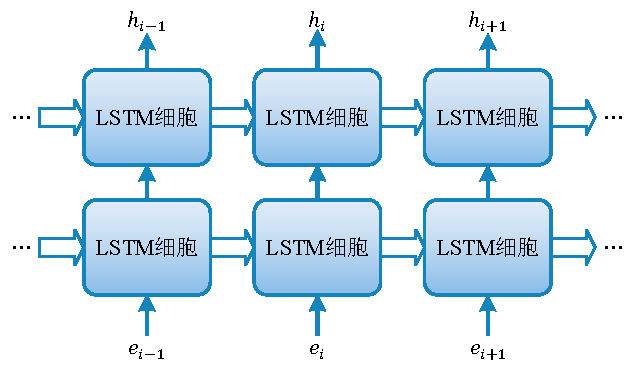
\includegraphics{deep-LSTM}
	\caption{深层 LSTM}
	\label{f:deep lstm}
	\vspace{-1em}
\end{figure}

\BiSubsection{分类结果生成}{}
LSTM 网络的输出向量最终需要转换为一个二元的输出 $y' \in \{0, 1\}$,考虑到使用连续变量能够更容易进行运算,本课题使 $y' \in [0, 1]$。

本课题中使用逻辑回归来完成上面的任务。逻辑回归函数如公式 (\ref{e:logit}) 所示:
\begin{equation}
F(x) = \frac{1}{1 + e^{-(\beta_0 + \beta_1 x)}}
\label{e:logit}
\end{equation}
其中 $\beta_0$ 与 $\beta_1$ 都是可训练参数。本课题取 LSTM 网络的最后一个输出为整个网络的输出向量,并应用逻辑回归函数得到分类结果。即:
\begin{equation}
y' = F(h_{|s|})
\end{equation}

为了提高模型性能,本课题还尝试在 LSTM 输出后增加一个全连接层。此时输出的二分类结果如下:
\begin{equation}
y' = F\bigl(\sigma(W_\text{full} h_{|s|} + b_\text{full})\bigr)
\end{equation}

\BiSubsection{模型训练}{}
\label{s:classifer p-training}
为了训练一个深度学习,需要定义一个损失函数,并且使用一种优化方法来最小化损失函数的值。

损失函数是一种用于衡量预测值 $y'$ 与真实值 $y$ 之间的偏差的函数。当 $y' = y$ 时,$L(y', y) = 0$;而当 $y' \neq y$ 时,$L(y', y) > 0$。一般而言,预测值与真实值之间的偏差越大,损失函数的值也应越大。这样使用数值优化的方法来最小化损失函数的值,就可以得到预测更为真实的模型。

在损失函数的选择方面,本课题选择了二分类问题常用的对数损失函数。对数损失函数的形式如下:
\begin{equation}
L(y', y) = -\bigl(y \log(y') + (1 - y) \log(1 - y')\bigr)
\end{equation}

由于采样句的数量可能与原句不相等,因此会形成不平衡数据集。为了将数据集平衡化,在汇总训练数据的损失函数值时应为每个训练数据赋予一个权重 $y(k - 1) + 1$。其中,$k$ 是训练集中采样居与原句的比例。这样,原句和采样句在训练中占有的权重就是相等的了。最终汇总的损失函数值如下:
\begin{equation}
\sum\bigl(y(k - 1) + 1\bigr) L(y', y)
\end{equation}

深度学习模型的训练大多使用基于梯度下降的优化算法。传统的随机梯度下降方法需要人为指定一个学习速率,并且在训练中途还可能需要进行学习速率的调整,这会给实验带来更多的麻烦。而一些自适应学习速率的优化算法则可以在学习过程中自行调节学习速率,例如 Adagrad\citeup{Duchi2011}、Adadelta\citeup{Zeiler2012}、RMSprop\footnote{RMSprop 并不是一个在论文中发表的算法,它是在多伦多大学的一个课堂讲义(\url{http://www.cs.toronto.edu/~tijmen/csc321/slides/lecture_slides_lec6.pdf})中被提出的。}与 Adam\citeup{Kingma2014}。为了降低实验的复杂程度,本课题使用了 \cite{Ruder2016} 中推荐的 Adam 算法进行模型训练。

\BiSection{程序实现}{}
\label{s:classifer implementation}
为了完成深度学习的二分类方法,本项目实现了一个可以处理原始语料、构建模型并进行训练的系统,其结构如图 \ref{f:classfier overall} 所示。
\begin{figure}[h]
	\centering
	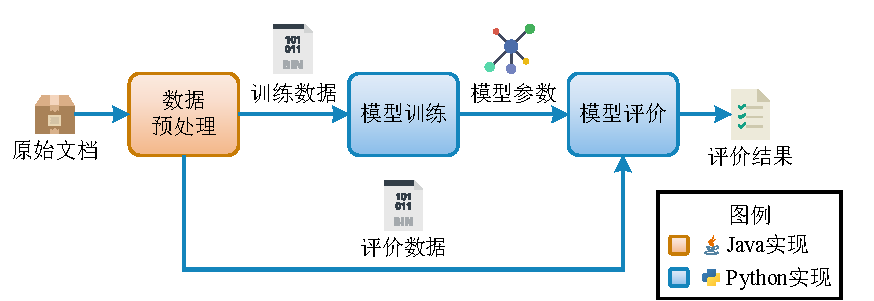
\includegraphics{Cl-overall}
	\caption{整体结构}
	\label{f:classfier overall}
	\vspace{-1em}
\end{figure}

程序实现分为数据预处理、模型训练和模型评价三个模块,根据模块特点的不同,分别使用了 Java 和 Python 两种编程语言实现。

\BiSubsection{数据预处理}{}
\label{s:classfier preprocess}
由于 Python 的文本处理性能较差,会花费过长的时间,数据预处理的程序使用 Java 语言编写。预处理程序的结构如图 \ref{f:classfier preprocess} 所示。

\begin{figure}[h]
	\centering
	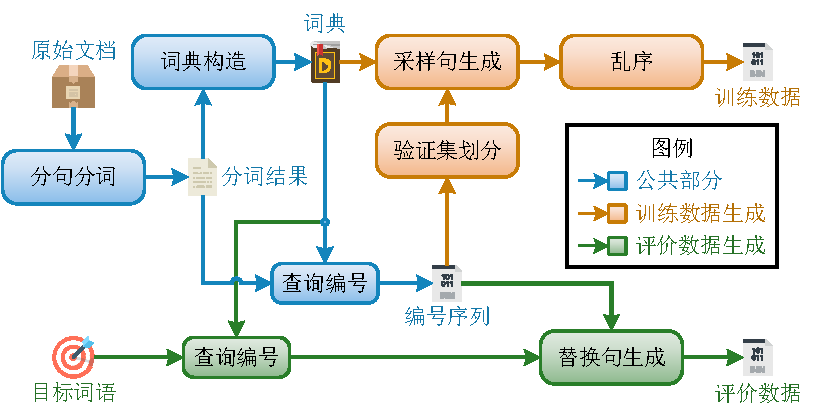
\includegraphics{Cl-preprocess}
	\caption{数据预处理}
	\label{f:classfier preprocess}
	\vspace{-1em}
\end{figure}

本课题使用了清华大学 THUCTC 工具包中提供的 THUCNews 数据集\citeup{Sun2016}作为语料库。该语料库中的内容为从新浪新闻中得到的新闻文档,属于无标注的生语料库,以文本形式存储在文件中。

为了提高模型的准确度,本课题的深度学习模型没有采用一些早期深度学习工作中常用的直接将文档切分为固定长度序列的方式,而是以句为单位进行训练。句子的识别只需要根据简单的标点符号规则,本课题最初实现的句子分割器与后来使用的 LTP 平台均是如此实现。

接下来对句子进行分词和词性标注。本课题尝试了多种现有的分词工具,包括 Java 语言的 Ansj,ltp4j 与 Python 语言的结巴分词。经过对比分词工具对测试集中词语的切分准确度,最终确定使用 Ansj 的 NLP 分词模式。由于部分分词工具的运行速度十分缓慢,分词和词性标注的结果以序列化的方式存储在磁盘上,以备后续步骤使用。

分词和词性标注的结果会被程序读取两次。第一次读取的目的是构造词典,由于词汇量过大,会对词嵌入步骤带来严重的麻烦,本课题将词典中词语的数量限制在 500000 个,超出词典大小的词语以它们的词性来代替。为了方便词嵌入,词典中的每个词语均赋予一个整数编号。第二次读取数据则是为了将词语序列转换为编号序列,以备后续步骤使用。

生成的序号序列会按照比例随机划分为训练集和验证集。训练集和验证集的后续处理步骤相同。

采样过程如上文中采样句的定义所述,会随机挑选被替换词和替换用词进行替换。在实际实验中,每个原句产生了 5 个采样句。

为了使学习的结果更加稳定,上述步骤得到的结果最终会被乱序处理。由于数据量过大,乱序处理无法在内存中进行。因此本课题使用了外存储器辅助完成乱序,如算法 \ref{a:shuffling} 所述。

\begin{algorithm}[h]
	\KwData{待乱序序列 $X$}
	\KwResult{乱序后序列 $Y$}
	\For{$i$ in $[1, n_\text{split}]$}{
		以写入模式打开临时文件 $F_i$\;
	}
	\For{$x$ in $X$}{
		设 $i$ 为 $1$ -- $n_\text{split}$ 之间的随机数\;
		将 $x$ 写入 $F_i$\;
	}
	\For{$i$ in $[1, n_\text{split}]$}{
		以读取模式重新打开 $F_i$\;
		从 $F_i$ 中读取全部内容 $Y_\text{split}$\;
		在 $Y_\text{split}$ 上执行内存乱序算法\;
		\For{$y$ in $Y_\text{split}$}{
			输出 $y$\;
		}
	}
	\caption{外存储器乱序算法}
	\label{a:shuffling}
\end{algorithm}

为了方便基于 TensorFlow 框架的 Python 程序读取数据,数据预处理阶段使用 TFRecords 格式保存数据。这样就可以避免书写 Python 程序读取数据,而通过 TensorFlow 中定义的 reader 来完成,避免数据的读取成为速度瓶颈。

\BiSubsection{模型训练}{}
\label{s:classifer training}
模型训练使用了 Python 语言的 TensorFlow 框架。该框架既可以通过简洁的 API 直接生成神经网络层,也可以使用基本操作对数据进行运算和调整。在运行时,TensorFlow 框架运用了 CUDA 技术,可以充分利用计算机的 GPU 资源。

为了平衡训练的速度和稳定性,各类基于梯度下降的学习算法往往需要将数据划分为 mini-batch,而每一个 mini-batch 的数据在 TensorFlow 平台中由一个多维数组来表述。这意味着在生成 mini-batch 时,需要将变长序列填补成固定长度的序列。利用 TensorFlow 框架提供的队列机制可以完成这一任务,它可以在取出内容时动态填补序列。每个序列需要一个单独的线程进行驱动。

使用 TensorFlow 框架开发程序的第一个步骤是数据读取。由于数据预处理程序已经将数据输出为 TFRecords 格式,这里可以使用 reader 轻松地读取数据。

接下来应构建 TensorFlow 图。TensorFlow 图由一系列的操作组成。每个操作接受一定数量(也可能没有)的 Tensor 作为输入,并且产生一个 Tensor 作为输出。TensorFlow 框架提供了包括 Tensor 变形、数学运算、神经网络层等 API 来应用操作。根据第 \ref{s:classifer pricinple} 节中所列出的表达式,就可以构造出完整的 TensorFlow 图。在构造过程中,应该注意设置设备布局,将适合 CPU 计算的操作布局在 CPU 上布局,而将适合 GPU 计算的操作在 GPU 上布局。

为了简化程序的编写,TensorFlow 框架提供了 Supervisor 机制以管理训练过程。Supervisor 负责产生驱动队列的线程,保存模型参数,并 TensorBoard 数据。创建 Supervisor 后,程序根据当前训练步数决定运行训练数据或验证数据。

\BiSubsection{模型评价}{}
为了评价模型,在数据的预处理阶段就需要根据目标词对生成用于评价的替换句。为了编程方便,评价数据的生成与训练数据的生成同时进行,这样很多用于训练数据生成的代码和中间数据都可以复用。程序只需要过滤所有的原句,查找目标词语。如果发现目标词语,则用词语对中对应的词语生成替换句。评价数据的数据格式与训练数据大致相同,只需要将原本的正负例标注换成用于生成替换句的词语对 ID。由于评价数据不影响模型训练,因此无需进行乱序操作。

将评价数据输入第 \ref{s:classifer training} 小节中构建的深度学习模型中,就可以得到每个句子的预测值 $y'$,这样,用于 TensorFlow 图构建的大部分程序可以被复用。根据词语对 ID 将预测值分组,并且求预测值的平均值,就可以得到每个词语对的相似度评价。对于词典外词汇,由所有句子的预测值平均值代替本词语对的预测值平均值。由于模型性能的评价指标是 Spearman 等级相关系数,与预测值的绝对值无关。因此无需对输出做任何缩放处理。Spearman 等级相关系数的计算由 Excel 软件完成。

\BiSection{实验结果}{}
本章所使用的实验环境如表 \ref{t:hw environment} 与表 \ref{t:sw environment} 所示。深度学习实验共进行了两次,分别采用不同的参数。其结果如表 \ref{t:classifer result} 所示。
\begin{table}[h]
	\caption{硬件环境}
	\label{t:hw environment}
	\vspace{0.5em}\centering\wuhao
	\begin{tabular}{cccc}
		\toprule[1.5pt]
		CPU & 内存 & 显卡 & 硬盘 \\
		\midrule[1pt]
		Intel Xeon E3-1230 & 16GB & NVIDIA Tesla K40c & 240GB SSD \\
		\bottomrule[1.5pt]
	\end{tabular}
\end{table}

\begin{table}[h]
	\caption{软件环境}
	\label{t:sw environment}
	\vspace{0.5em}\centering\wuhao
	\begin{tabular}{ccccc}
		\toprule[1.5pt]
		操作系统 & CUDA 版本 & cuDNN 版本 & TensorFlow 版本 & Python 版本 \\
		\midrule[1pt]
		Ubuntu 16.04 & 8.0 & 5.1 & 1.1.0 & Python 3.6 (Miniconda 3) \\
		\bottomrule[1.5pt]
	\end{tabular}
\end{table}


\begin{table}[h]
	\caption{实验结果}
	\label{t:classifer result}
	\vspace{0.5em}\centering\wuhao
	\begin{tabular}{cccccc}
		\toprule[1.5pt]
		词嵌入维数 & LSTM 单元数 & LSTM 层数 & 全连接层数 & 损失函数值 & \makecell{Spearman \\ 等级相关系数} \\
		\midrule[1pt]
		300 & 128 & 2 & 0 & 0.5422 & 0.1313 \\
		300 & 300 & 3 & 0 & 0.5972 & 0.1484 \\
		300 & 128 & 2 & 1 & 0.5448 & 0.1579 \\
		\bottomrule[1.5pt]
	\end{tabular}
\end{table}

从实验结果中可以看出,适当增加 LSTM 单元数和层数,可以提高模型的最终性能,但这种性能提高少于一个全连接层所能带来的。鉴于训练全连接层的代价要小于 LSTM 层,因此后者是优化模型的有效方式。然而,三次训练得到的模型成绩都不是很高,这意味着深度学习的二分类模型并不适合单独用于解决词语相似度问题。尽管如此,这种方法输出的信息对于本课题后期的集成学习仍然是有正面意义的。

三次训练的损失函数下降情况如图 \ref{f:classifer loss} 所示,其中横坐标是训练的轮数,而纵坐标是损失函数值。可以看出,三次训练中损失函数值均已收敛。

\begin{figure}[h]
	\centering
	\subfigure[第一次训练]{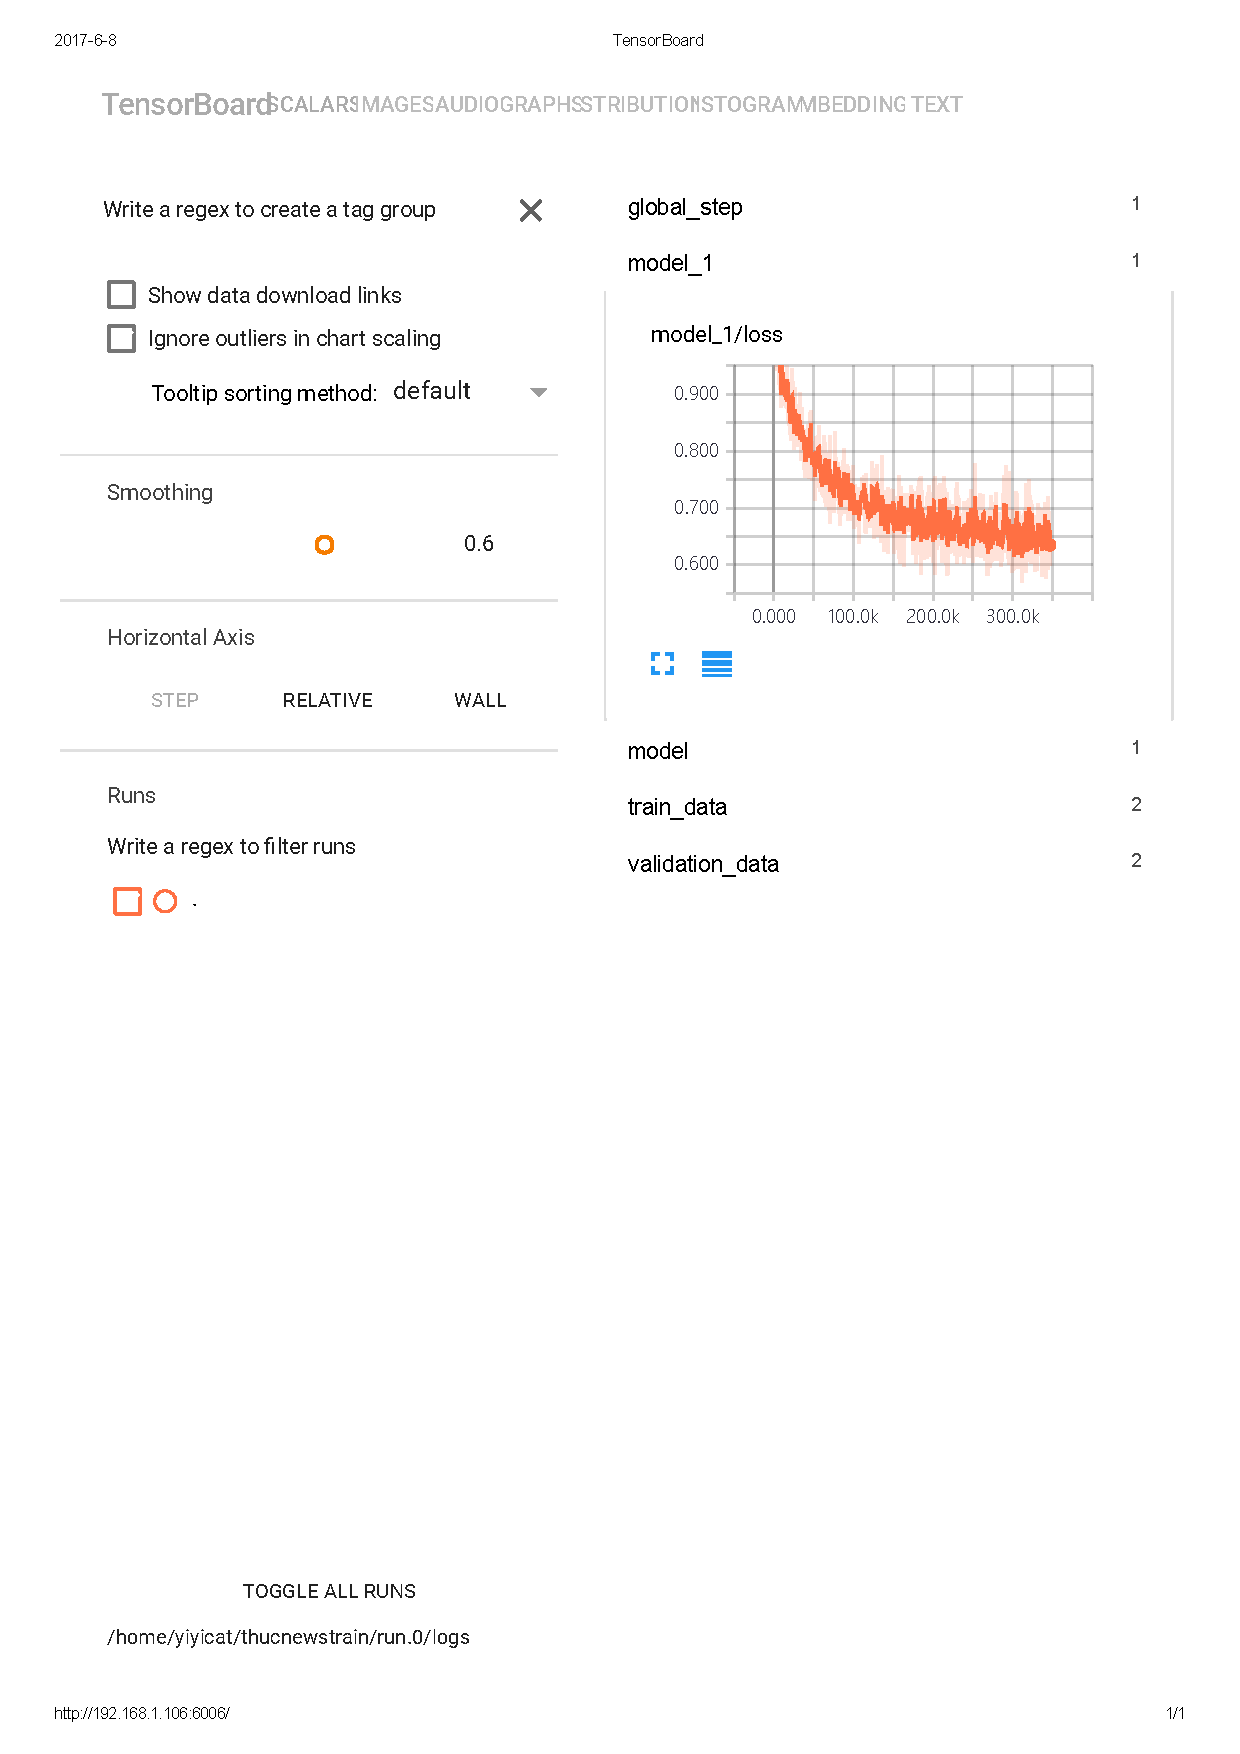
\includegraphics[trim={11.35cm 19.1cm 2.4cm 6.1cm},clip]{Cl-train1}}
	\subfigure[第二次训练]{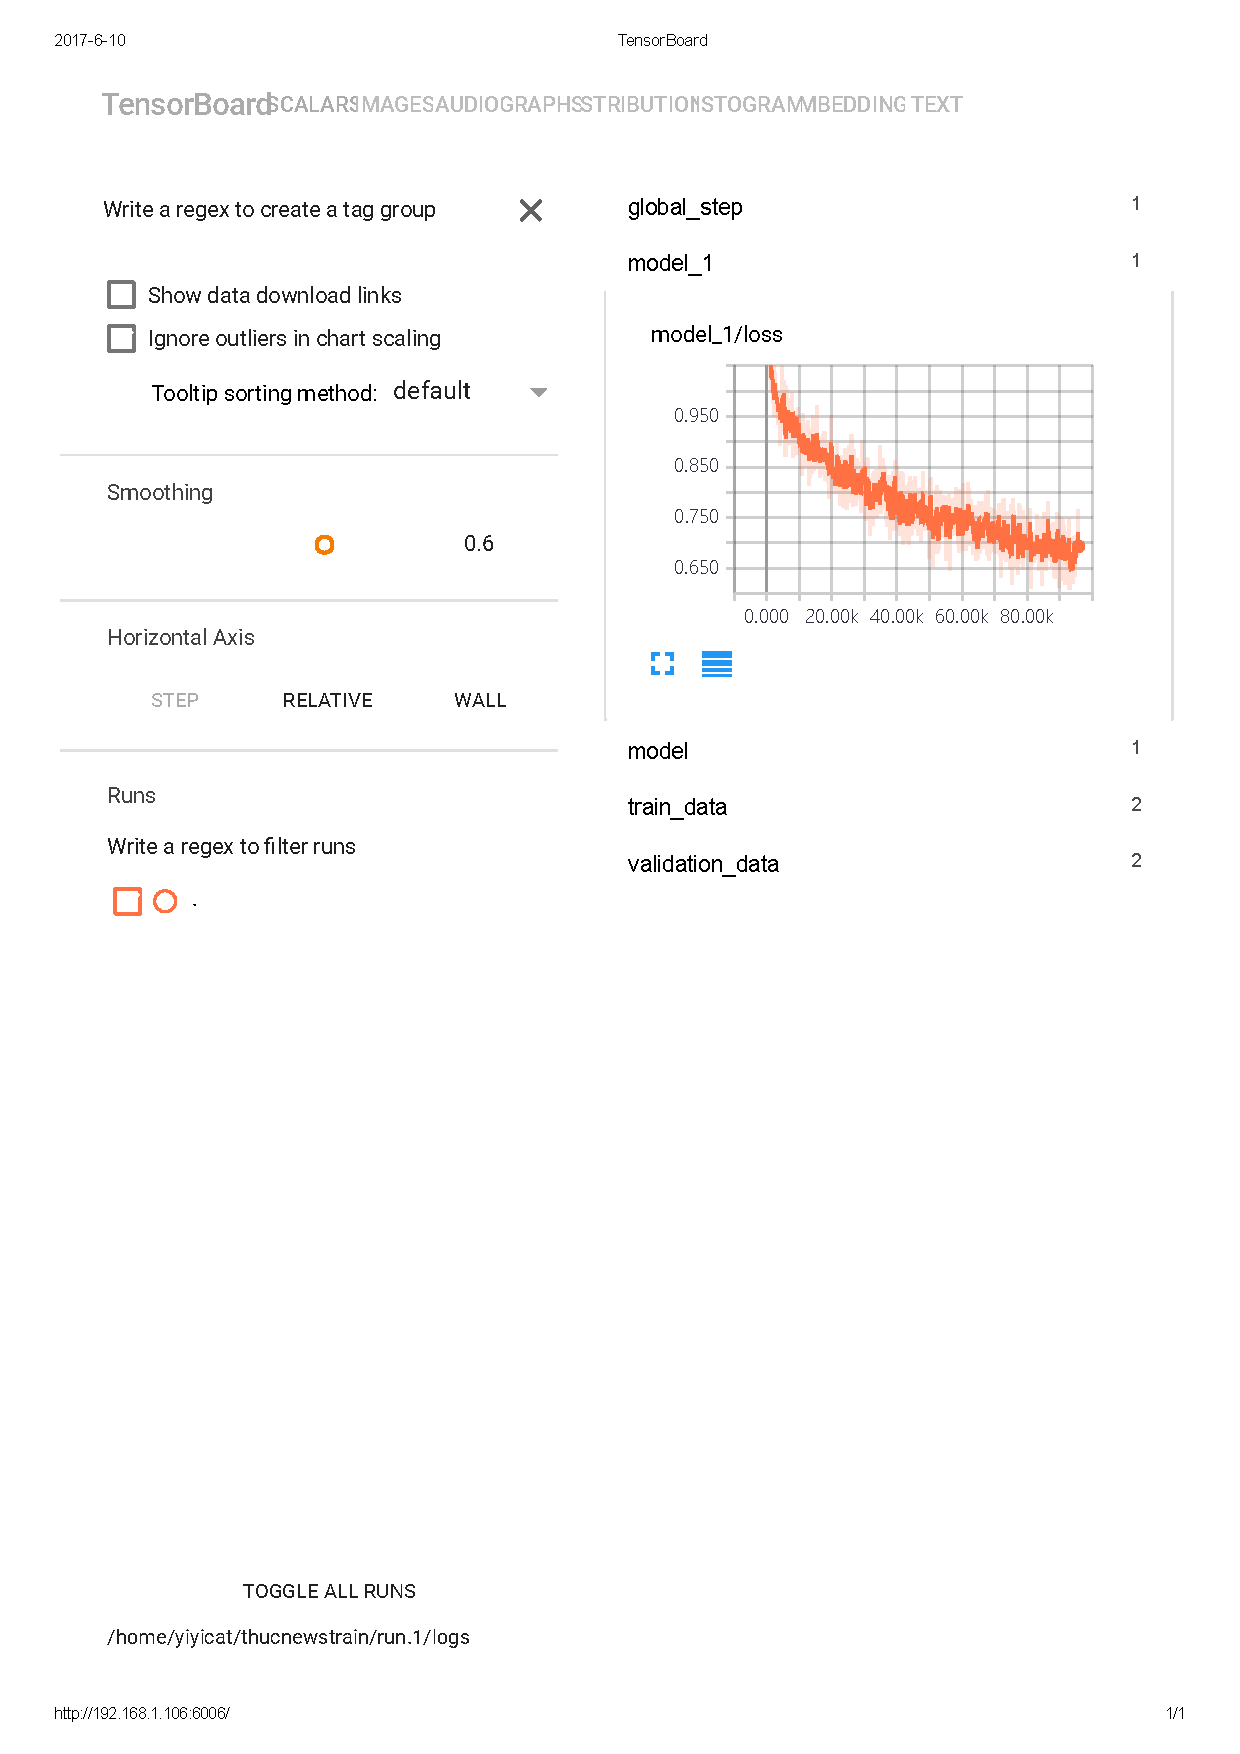
\includegraphics[trim={11.35cm 19.1cm 2.4cm 6.1cm},clip]{Cl-train2}}
	\subfigure[第三次训练]{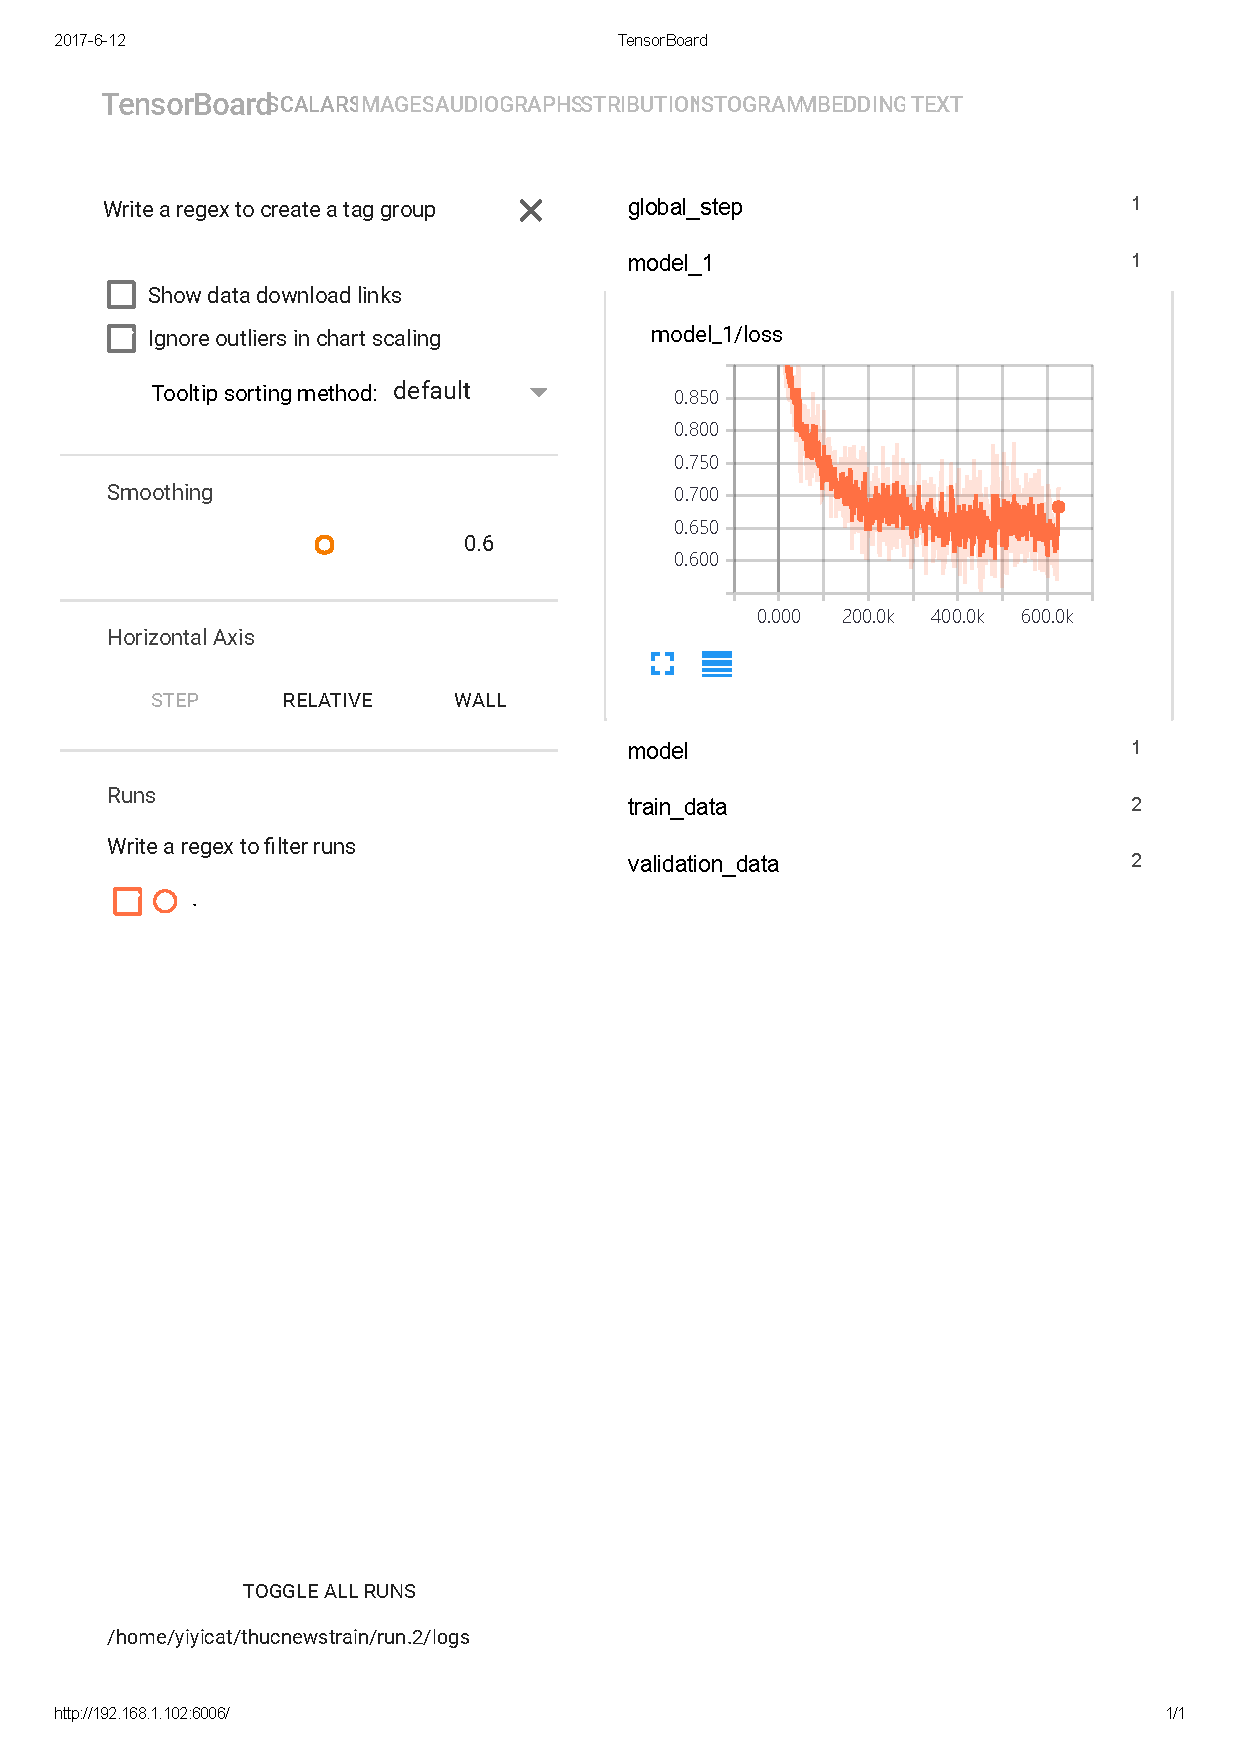
\includegraphics[trim={11.35cm 19.1cm 2.4cm 6.1cm},clip]{Cl-train3}}
	\caption{损失函数下降情况}
	\label{f:classifer loss}
	\vspace{-1em}
\end{figure}
% !Mode:: "TeX:UTF-8" 

\BiChapter{绪论}{}
\BiSection{问题背景}{}
词语的相似度计算是自然语言处理中的一项基本任务。它的目的是使用自动化的方法给出一个量化的指标,来衡量一对词语之间的相似程度。词语相似度计算对于很多高层次的自然语言处理任务有着重要的意义,例如问答、信息检索、改写检测与文本蕴含。

为了评价一种词语相似度计算方法的好坏,可以使用内部任务评价或外部任务评价。内部任务评价直接使用一个标准的词语相似度标注数据集,并使用一些评价指标来衡量机器给出的结果与标准数据集之间的差异;而外部任务评价则利用词语相似度计算的结果解决其他的高层次机器学习问题,通过衡量不同计算结果在这些问题上的性能来简介衡量词语相似度计算方法的好坏。

本课题取自 NLPCC-ICCPOL 2016 会议中的“中文词语相似度计算”开放任务。该开放任务使用内部任务评价的方式来衡量各参赛队提交的结果。其组织者发布了一个 PKU-500 数据集\citeup{Wu2016},其中包含 500 个词语对,以及对每个词语对之间的相似度标注。共有 49 个参赛队伍报名参加了此次开放任务,而最终由 21 个参赛队伍提交了总计 24 个系统\citeup{Wu2016}。

\BiSection{相关工作}{}
在英文词语相似度任务中,已经有多个数据集可以作为基准测试。其中,使用最广泛的是 WordSim-353 数据集。这个数据集包含 353 个词语对,并由 16 名标注者对其相似度进行了标注。

在 NLPCC-ICCPOL 2016 会议举办之前,Semeval-2012 会议上也举行了一次中文词语相似度的比赛,比赛所使用的词语对是经过翻译的 WordSim-353 数据集,并重新进行了人工标注。遗憾的是,这次比赛只有两个队伍参加。

本次开放任务中的参赛队伍使用的方法大致分为三类:基于辞典或知识库的方法、基于语料的方法与基于信息检索的方法。

基于词典或知识库的方法利用了一些现有的语言学资源,例如知网(HowNet)和同义词词林。这些词典或知识库的作者往往同时给出了用于计算词语相似度的规则。有些参赛队伍直接使用了这些规则,还有一些对这些规则进行了修改。这些方法依赖于词典或知识库的组织结构,并且无法处理未登录词。此外,人工制定的规则是否合理也是影响模型性能的重要因素。

基于语料的方法主要是根据上下文信息进行词嵌入,这类方法假设“相似的词语应该出现在相似的上下文中”。典型的词嵌入方法,例如 word2vec,具有成熟的工具包,因此在各参赛队伍中非常受到欢迎。除了词嵌入方法以外,来自大连理工大学的参赛队\citeup{Pei2016}使用了深度学习的方法来识别描述词语类比的句子,例如“寂寞和孤单的区别是什么”。如果这类句子出现在语料中,很可能意味着这两个词语是相关的。基于语料的方法需要大规模的语料库和漫长的训练时间,由于这些模型普遍使用无需人工标注的生语料库,因此语料的获取来源非常广泛。而训练时间的缩短只能通过使用运算能力更强的硬件,因此实验可能受到硬件条件的制约。针对中文语料而言,绝大部分的模型是以词为单位进行处理,这样分词的准确度也会对模型最终性能产生一定影响。

基于信息检索的方法利用搜索引擎查询包含目标词语的页面,根据同时包含两个词语的页面数、仅包含一个词语的页面数利用公式计算目标词语的相似度。这种方法的实现非常的简单,只需爬取搜索引擎的结果页面,或调用搜索引擎提供的 API。有的队伍将这种方法作为多种评价方法之一\citeup{Ma2016},也有的队伍用信息检索得到的结果作为弱监督学习的指标\citeup{Pei2016}。这种方法的一大问题是词语相似度和词语共同出现的频率并不一致,例如一些事物的别名经常在科普类的文章中被介绍(例如“西红柿”和“番茄”),而因口语习惯而导致不同的同义词(例如“拖后腿”和“拉后腿”)就很难在一篇文章中同时出现\citeup{Zhang2017}。

\BiSection{数据生成与评价指标}{}
PKU-500 数据集的生成过程分为三个步骤,分别为词语选择、词语对生成和相似度标注。

PKU-500 数据集的词语选择过程遵循以下的条件:
\begin{enumerate}
	\item 领域:同时涉及传统书面语言与近期的网络语言。
	\item 频率:应同时包含高频、中频与低频的词语。
	\item 词性:应同时包含名词、动词与形容词。除上述实词外还应包含虚词(例如副词和连词)。
	\item 字数:应包含 1 -- 4 个字的词语。
	\item 词义:应包含部分多义词。
	\item 极性:应同时包含正面词语与负面词语。
\end{enumerate}
根据上述条件,词语的选择过程如下:
\begin{enumerate}
	\item 数据来源于两个领域:三个月的《人民日报》新闻与一大批新浪微博数据。
	\item 数据经过开源的 Ansj 工具进行分词和词性标注。
	\item 从两个领域中分别根据其频率、词性与字数抽取词语。
	\item 根据词义与极性手动挑选自动抽取的词语,最终从《人民日报》新闻与微博数据中分别得到了 514 和 202 个词语。
\end{enumerate}

上述步骤生成了 716 个单独的词语,接下来的步骤用于生成词语对:
\begin{enumerate}
	\item 对于每一个词语,从哈工大同义词词林(扩展板)中自动提取三个候选词语:第一个属于同一个原子词群,第二个属于某一个父节点,第三个是从其它词语中随机选择的。
	\item 每个目标词语的候选词语被进一步人工挑选,并根据上文中提到的条件去除与增加了一些词语,最终得到 470 个词语对。
	\item 从 WordSim-353 数据集中选择 30 个翻译的词语对。
	\item 最终,得到了 500 个用于中文词语相似度计算的词语对。
\end{enumerate}

相似度标注过程由 20 个研究生完成,他们都以中文为母语,来自汉语言学专业。相似度的取值范围为 $[1, 10]$,其中 1 表示词语完全不同,而 10 表示词语意义相同。最终的相似度得分是 20 个人类标注的平均值。标注者没有受到任何有关标注的指示,这意味着他们会根据自己对语言的理解来判断。同时,对相关性与相似度也不加区分。

上述过程得到的 500 个词语对全部作为测试数据,而不提供训练数据。在开放任务开始前,组织者先行公布了 40 个词语对作为样例。参赛系统可以使用任何技术,例如传统的基于语料分布的相似度、基于词典的相似度,与近期发展出来的词嵌入与深度学习方法。

为了防止对小数据集的过拟合,该开放任务的组织者将 500 个词语对混入了 10000 个从大词典中随机生成的词语对,并作为参赛系统的输入。

系统性能的评价指标是系统输出与人工标注之间的 Spearman 等级相关系数:
\begin{equation}
\rho = 1 - \frac{6 \sum_{i = 1}^{n}(R_{X_i} - R_{Y_i})^2}{n(n^2 - 1)}
\end{equation}
其中,$n$ 是词语对的数量,而 $R_{X_i}$ 与 $R_{Y_i}$ 分别是系统输出与人工标注相似度的等级变量(排名)的标准差。

\BiSection{本课题研究方法}{}

本课题的主要研究四种方法。一是深度学习的二分类方法,二是深度学习辅助词嵌入方法,三是基于词典或知识库的方法,四是集成学习方法。上述方法或直接用于词语相似度计算,或用于改进与结合现有的方法。

\BiSubsection{深度学习的二分类方法}{}
将困难问题规约到简单问题是科学研究中常用的手法,本方法将词语相似度计算这一无监督回归问题转化为有监督分类问题,以降低解决问题的难度。对于句子的分类问题,本方法使用循环神经网络以及它们的变种 LSTM 予以解决。

\BiSubsection{深度学习辅助词嵌入方法}{}
词嵌入是自然语言处理中的一项非常成熟的技术,它可以将词语映射到向量空间中。而向量具有天然的相似度评价方法,这使得词嵌入技术经常被用于解决词语相似度计算问题。本方法查找现有词嵌入技术中的局限性,并使用深度学习方法拓展现有词嵌入技术,以改善它们的性能。

\BiSubsection{基于词典或知识库的方法}{}
很多现有的语言学资料中提供了对词语语义的一些形式化的解释。这些解释可以被计算机解析和利用,因此也可以作为词语相似度计算的素材。本方法尝试使用现有的词典或知识库资源,并对业界常用的利用它们进行词语相似度计算的方法进行一些改进。

\BiSubsection{集成学习方法}{}
实际的词语相似度计算系统多是多种方法的结合。这有助于发挥各方法的长处,同时提高系统的稳定性。在其它开放任务参赛队发表的系统中,集成多种技术最常见的方法是简单平均法和加权平均法。除此之外,很多人为制定的基于规则的结合策略也被用于此用途。这些方法虽然简单朴素,甚至有些看起来缺乏理论根据,但是在词语相似度计算的任务中取得了相当优秀的成绩。尽管如此,发现一个好的结合规则仍然需要大量实验和一定的运气成分。因此,需要借助集成学习的技术来发现一种更可靠的、表现更为稳定的方法。
\include{body/figures}
\include{body/tables}
\include{body/equations}
% !Mode:: "TeX:UTF-8" 

\BiChapter{模板的其它说明}{Other explanation about the template}

\BiSection{中英文封面的相关信息}{Related information in Chinese and English covers}
国内图书分类号(Classif\/ied Index)的查询网址:

\centerline{\href{http://www.ztflh.com/}{http://www.ztflh.com/}——中国图书馆分类法}
国际图书分类法(U.D.C)的查询网址:

\centerline{\href{http://www.udcc.org/udcsummary/php/index.php}{http://www.udcc.org/udcsummary/php/index.php}——UDC Summary}
学校代码查询网址:

\centerline{\href{http://www.marry360.com.cn/Tools/UniversityCodeList.aspx}{http://www.marry360.com.cn/Tools/UniversityCodeList.aspx}——高校代码查询}
\noindent 哈尔滨工业大学的学校代码为~10213。

英文封面下方的学位论文相关信息可以采用~\verb|tabular|~和~\verb|tabularx|~两种表格环境,具体使用哪一种环境和具体的相关信息有关。若信息内容不太长,不会引起信息内容分行时,则应该采用~\verb|tabular|~环境;若信息内容过长,会引起信息内容分行时,则应该采用~\verb|tabularx|~环境。具体用法请见~format.tex~文件的相应代码。

\BiSection{\textsc{Bib}\kern-.08em\TeX~文献文件的写法}{How to write the \textsc{Bib}\kern-.08em\TeX~bibliographic file}
用在~\LaTeX~中的~\textsc{Bib}\kern-.08em\TeX~文献文件的扩展名为~bib,此模板中,该文件即为~reference.bib。bibtex.exe 命令根据~GBT7714-2005NLang-HIT.bst 文件定义的文献格式,将~reference.bib 中的文献数据转换为输出文档中的文献列表。GBT7714-2005NLang-HIT.bst 文件是在~\href{http://bbs.ctex.org/attachment.php?aid=MjA3MDh8ZDcyMjc2MTN8MTMyNTYzNjY4OHxhZTg4bkNCUVJiRzA0WmU3TmlMbVdTUVExa0xtV2puWWc0dkdqbVJhbTVMdy9mVQ\%3D\%3D}{GBT7714-2005NLang-UTF8.bst} 文件的基础上修改得到的,所做的唯一一处改动是将姓氏字母全部大写的英文作者名改为只首字母大写,以保证和\href{http://219.217.226.141/xuewei/guifan.doc}{《研究生学位论文撰写规范》}及其\href{http://219.217.226.141/xuewei/fanli.doc}{《研究生学位论文书写范例》}相一致。

bib 文件的编写方法可参考模板中已给出的例子,也可参考~\href{http://bbs.ctex.org/attachment.php?aid=MTk3OTd8NjY1ODc5OGV8MTMyNTY0MTEyMnxhZGZkYWpsa0I2RGZwNDR5Z1lyeStjb1dKRS8rTnJub3lvT2FkNDNJbHl1UWVkVQ\%3D\%3D}{GBT7714-2005.bst说明文档20060919
} 中所给出的例子。

中文文献需要添加一个额外的~language 域,并使得域值非空,这样~bst 文件就能够判断此文献为中文文献,进而能正确地生成参考文献格式。

GBT7714-2005.bst 对于国标~GB/T 7714-2005 的文献分类如表~\ref{tab:entrytypes} 所示。对于每种文献类型的缺省类型,已经设置好相应的文献标识码,因此不需要输入相应的文献
标识码。扩展类型的文献则应再添加一个~TypeofLit 域,并需要将其域值改为相应的文献标识码。
\begin{table}[htbp]
\bicaption[tab:entrytypes]{}{GBT7714-2005.bst 的分类方式}{Table$\!$}{Classification method of GBT7714-2005.bst}
\vspace{0.5em}\centering\wuhao
\begin{tabular}{llll}
\toprule[1.5pt]
文献类型 & 缺省类型 & 扩展类型(需要手 & 主要特征\\
 &  & 工加入文献标识码) & \\
\midrule[1pt]
article & 文章[J] & 报纸中的析出文献[N] & 年,卷(期):页码\\
 &  & 在线文章[J/OL] & \\
book & 书[M] & 论文集、会议录[C] & \\
 &  & 在线书[M/OL] & \\
 &  & 汇编[G] & \\
inbook & 书的某几页[M] &  & \\
incollection & 书中析出的文章[M]// & 汇编的析出文献[G]// & 析出文献[文献标识码]//\\
 &  & 标准的析出文献[S]// & \\
proceedings &  &  & \\
inproceedings & 论文集、会议录中的 & 在线论文集、 & 析出文献[文献标识码]//\\
/conference & 析出文献[C]// & 会议录[C/OL]// & \\
mastersthesis & 毕业论文[D] &  & 类似book类\\
phdthesis & 毕业论文[D] &  & 类似book类\\
techreport & 科技报告[R] &  & 类似book类\\
misc &  & 杂项[],例如:专利[P] & 此类一般是网上文件,\\
 &  & 网上专利[P/OL] & 按照国标规定顺序\\
 &  & 网上电子公告[EB/OL] & 编码制时不输出年份\\
 &  & 磁盘[CP/DK] & \\
\bottomrule[1.5pt]
\end{tabular}
\end{table}

《研究生学位论文撰写规范》及《研究生学位论文书写范例》中所列英文参考文献例子中的文章名的每个实词首字母都大写,因此需要将英文参考文献的~title 域手动修改为每个实词首字母大写。

英文参考文献在~author 域中的作者名需要将姓置前,名置后。

\BiSection{参考文献的引用}{Citation of references}
需要将~main.tex 文件中的语句~\verb|\nocite{*}| 屏蔽掉,这样,文中未引用的参考文献就不会出现在文后的参考文献列表中。文中参考文献的引用方法:

\begin{itemize}
\item 行文引用请使用命令~\verb|\cite{引用词}|;
\item 上标引用请使用命令~\verb|\citeup{引用词}|。
\end{itemize}
其中,上标引用命令~\verb|\citeup{}| 为本模板自定义的命令,其定义为
\begin{verbatim}
\newcommand{\citeup}[1]{\textsuperscript{\cite{#1}}}
\end{verbatim}

\BiSection{单层罗列环境}{Monolayer list environment}
哈工大学位论文一般可采用两种罗列环境:一种是并列条目有同样标签的~\verb|itemize|~罗列环境,另一种是具有自动排序编号符号的~\verb|enumerate|~罗列环境。这两种罗列环境的样式参数可参考图~\ref{list}。
\begin{figure}[htbp]
\centering
\includegraphics[width = 0.6\textwidth]{list}
\bicaption[list]{}{罗列环境参数示意图}{Fig.$\!$}{Schematic diagram of list environments}\vspace{-1em}
\end{figure}
通过调用~enumitem~宏包可以很方便地控制罗列环境的布局,其~format.tex~文件中的~\verb|\setitemize|~和~\verb|\setenumerate|~命令分别用来设置~\verb|itemize|~和~\verb|enumerate|~环境的样式参数。采用~\verb|itemize|~单层罗列环境的排版形式如下:
\begin{itemize}
\item 第一个条目文本内容
\item 第二个条目文本内容
\item 第三个条目文本内容
\end{itemize}
其代码如下
\begin{verbatim}
\begin{itemize}
  \item 第一个条目文本内容
  \item 第二个条目文本内容
  ...
  \item 第三个条目文本内容
\end{itemize}
\end{verbatim}
采用~\verb|enumerate|~单层罗列环境的排版形式如下:
\begin{enumerate}
\item 第一个条目文本内容
\item 第二个条目文本内容
\item 第三个条目文本内容
\end{enumerate}
其代码如下
\begin{verbatim}
\begin{enumerate}
  \item 第一个条目文本内容
  \item 第二个条目文本内容
  ...
  \item 第三个条目文本内容
\end{enumerate}
\end{verbatim}

\BiSection{算法}{Algorithm}

这是一个算法的例子,来自~worldguy@lilacbbs。建议将算法放在~minipage~环境中,避免算法出现在页面版心之外。

\begin{algorithm}
\KwIn{training samples, {$(d_i, d_j)_q$; $\mathbf{q}_i, \mathbf{q}_j \in C$,
$q\in \mathbf{Q}$} }
\KwOut{parameter setting $\lambda^T$}%

\For{$t$=1 to $T$}
{   
    $\lambda^{t+1}_n = \lambda^t_n + \eta (f_n(q, c, d_i) - f_n(q, c, d_j))$
 }
\end{algorithm}

%\KwIn{training samples, {$(d_i, d_j)_q$; $\mathbf{q}_i, \mathbf{q}_j \in C$,
%$q\in \mathbf{Q}$} }
%\KwOut{parameter setting $\lambda^T$}%
%
%\For{$t$=1 to $T$}
%{   
%    $\lambda^{t+1}_n = \lambda^t_n + \eta (f_n(q, c, d_i) - f_n(q, c, d_j))$
% }
%\end{algorithm}

算法环境中右侧空白比较多,若想把右侧的空白框减小,可以采用~minipage~环境实现。把~algorithm~环境放到~minipage~环境里面,并且加上选项[H]禁止算法浮动,下面给出一个例子。需要说明的是,一般不需要进行这种处理。算法标题可有可无,若有中英文标题,请使用~\verb|\AlgoBiCaption{中文标题}{英文标题}|。下面给出两个有标题的例子。需要说明的是,算法的标题是自动换行,没有必要手动换行。

\begin{minipage}{0.8\textwidth}\centering
\begin{algorithm}[H]
 \AlgoBiCaption{这是一个简短的算法中文图题}{This is the English caption of the algorithm}
  \KwIn{training samples, {$(d_i, d_j)_q$; $\mathbf{q}_i, \mathbf{q}_j
      \in C$, $q\in \mathbf{Q}$} }
 \KwOut{parameter setting
    $\lambda^T$}
 \For{$t$=1 to $T$} { $\lambda^{t+1}_n = \lambda^t_n +
    \eta (f_n(q, c, d_i) - f_n(q, c, d_j))$ }
\end{algorithm}
\end{minipage}


\begin{minipage}{0.9\textwidth}\centering
\begin{algorithm}[H]
 \AlgoBiCaption{这是一个算法的比较长的中文图题,需要换行,这里采用自动换行,如果手动换行会造成算法目录中同样出现断行}{This is a long English caption of the algorithm, a new line  required, and this a new line}
  \KwIn{training samples, {$(d_i, d_j)_q$; $\mathbf{q}_i, \mathbf{q}_j
      \in C$, $q\in \mathbf{Q}$} }
 \KwOut{parameter setting
    $\lambda^T$}
 \For{$t$=1 to $T$} { $\lambda^{t+1}_n = \lambda^t_n +
    \eta (f_n(q, c, d_i) - f_n(q, c, d_j))$ }
\end{algorithm}
\end{minipage}

\BiSection{定理定义}{Theorem and definition}

若需要书写定理定义等内容,而且带有顺序编号,需要采用如下环境。除了~\verb|proof|~环境之外,其余~9~个环境都可以有一个可选参数作为附加标题。

\begin{center}\vspace{0.5em}\noindent\wuhao\begin{tabularx}{0.7\textwidth}{lX|lX}
定理 & \verb|theorem|~环境 & 定义 & \verb|definition|~环境 \\
例 & \verb|example|~环境 & 算法 & \verb|algo|~环境 \\
公理 & \verb|axiom|~环境 & 命题 & \verb|proposition|~环境 \\
引理 & \verb|lemma|~环境 & 推论 & \verb|corollary|~环境 \\
注解 & \verb|remark|~环境 & 证明 & \verb|proof|~环境 \\
\end{tabularx}\end{center}

% !Mode:: "TeX:UTF-8" 

\BiAppendixChapter{结\quad 论}{Conclusions}

本课题得到了一套系统完整的中文词语相似度计算方法,其性能在已知的方法中处于较高的地位。高性能的词语相似度计算将会为多种下游自然语言处理问题提供可靠的保障。

深度学习的二分类方法创新性地将无监督回归问题转化为了有监督分类问题,使得广泛存在于互联网中的生语料库可以被用于词语相似度计算问题中。深度学习辅助词嵌入方法利用词嵌入技术解决了词语相似度计算问题,并使用双向LSTM改进了已有的ivLBL方法,充分将LSTM的序列学习能力运用到上下文向量的生成中,扩大了上下文的学习范围,使得词嵌入的质量得到显著的提升。基于或知识库的方法与集成学习方法相结合,改变了传统的基于规则组合特征的方式。集成学习方法有效地组合了上述方法的输出,并得到了比每个个体学习器更强的性能。

然而,本方法也有一定的不足之处。其中一个问题在于本方法无法处理词典外词汇,对于他们只能使用平均值等数据来填充。另一个问题在于集成学习的性能严重受制于有标注数据集的大小和质量。随着日后中文词语相似度标注数据集的增多,本方法的性能也会得到更大的提升。   % 结论

%\include{body/simplefigure}
%\include{body/simpletable}
%\include{body/simpleequation}
%\include{body/simplereference}


%参考文献
\defaultfont
\bibliographystyle{GBT7714-2005NLang-HIT}
\addcontentsline{toc}{chapter}{参考文献}      % 参考文献加入到中文目录
\addcontentsline{toe}{chapter}{\bfseries  References} % 参考文献加入到英文目录
\addtolength{\bibsep}{-0.8em}
\nocite{*}  %若将此命令屏蔽掉,则未引用的文献不会出现在文后的参考文献列表中。
\bibliography{reference}
% -*-coding: utf-8 -*-

\defaultfont
\appendix

\BiAppChapter{据说还要写文献翻译好气哦!}{}    % 附录
\include{appendix/publications}    % 所发文章
\ifxueweibachelor
  % !Mode:: "TeX:UTF-8" 

\BiAuthorization

本人郑重声明:在哈尔滨工业大学攻读学士学位期间,所提交的毕业设计(论文)《\chinesethesistitle》,是本人在导师指导下独立进行研究工作所取得的成果。对本文的研究工作做出重要贡献的个人和集体,均已在文中以明确方式注明,其它未注明部分不包含他人已发表或撰写过的研究成果,不存在购买、由他人代写、剽窃和伪造数据等作假行为。

本人愿为此声明承担法律责任。

\vspace{\baselineskip}
\hspace{6em}作者签名:\hfill 日期:\hspace{2.5em}年\hspace{1.5em}月\hspace{1.5em}日
 % 本科蛋疼承诺
\else
  \include{appendix/Authorization} % 硕博承诺
\fi   
% !Mode:: "TeX:UTF-8" 

\BiAppendixChapter{致\quad 谢}{Acknowledgements}
感谢我的毕业设计指导老师孙大烈老师和刘旭东老师在答辩和论文方面给予我的指导。

感谢我的硕士生导师李舟军老师教授我本课题中使用的关键技术。

感谢傅忠传老师为本课题的深度学习实验提供硬件平台,并感谢张源悍学长在硬件平台配置过程中提供的帮助。

感谢车万翔老师为本课题提供实验数据。

本课题使用了北京大学的 PKU-500 数据集、清华大学的 THUCNews 数据集以及哈尔滨工业大学的同义词词林扩展版,感谢这些数据集的作者做出的贡献。

论文的插图中使用了 \href{http://www.flaticon.com}{Flaticon} 网站中由 \href{http://www.flaticon.com/authors/madebyoliver}{Madebyoliver}、\href{http://www.freepik.com}{Freepik}、\href{http://www.flaticon.com/authors/roundicons}{Roundicons}、\href{http://www.flaticon.com/authors/vectors-market}{Vectors Market} 与 \href{http://www.flaticon.com/authors/maxim-basinski}{Maxim Basinski} 提供的图标资源,这些图标以 \href{http://creativecommons.org/licenses/by/3.0/}{CC 3.0 BY} 协议发布。

最后,感谢我最爱的人郭怡心,在我本科四年的生活中给予我的陪伴、鼓励与支持。% 致谢

\ifxueweidoctor
\include{appendix/Resume}          % 博士学位论文有个人简介
\fi

\clearpage

\end{document} 